%%%%%%%%%%%%%%%%%%%%%%%%%%%%%%%%%%%%%%%%%%%%%%%%%%%%%%%%%%%%%%%%%
% Contents: The accounts chapter
% $Id: grisbi-manuel-accounts.tex, v 0.4 2002/10/27 Daniel Cartron
% $Id: grisbi-manuel-accounts.tex, v 0.5.0 2004/06/01 Loic Breilloux
% some of its content was in tips chapter: 
% $Id: grisbi-manuel-tips.tex, v 0.4 2002/10/27 Daniel Cartron
% $Id: grisbi-manuel-accounts.tex, v 0.6.0 2011/11/17 Jean-Luc Duflot
% some of its content was in tips chapter:
% $Id: grisbi-manuel-tips.tex, v 0.5.0 2004/06/01 Loic Breilloux
% $Id: grisbi-manuel-accounts.tex, v 0.8.9 2012/04/27 Jean-Luc Duflot
% $Id: grisbi-manuel-accounts.tex, v 1.0 2014/02/12 Jean-Luc Duflot
% some of its content was in transactions chapter:
% $Id: grisbi-manuel-transactions.tex, v 0.8.9 2012/04/27 Jean-Luc Duflot
% $Id: 07-grisbi-manuel-account-fr.tex, v 3.0 2026/01 Dominique Brochard

%%%%%%%%%%%%%%%%%%%%%%%%%%%%%%%%%%%%%%%%%%%%%%%%%%%%%%%%%%%%%%%%%

\chapter{Kontoverwaltung\label{accounts}}%Account management%Gestion des comptes

Grisbi kann vier Arten von Konten verwalten, deren Verwendung im Abschnitt \vref{accounts-type}, \menus{Kontoarten bei Grisbi}:
%Grisbi can manage four types of accounts, the use of which is described in detail in the section \vref{accounts-type}, \menus{Grisbi account types}:
%Grisbi sait gérer quatre types de compte, dont l'utilisation est décrite précisément dans la section \vref{accounts-type}, \menus{Types de compte de Grisbi}:
\begin{itemize}
	\item \indexword{Bankkonto}\index{Bankkonto}: Es ermöglicht Ihnen, jede Art von Buchhaltungsvorgang durchzuführen;
	% \indexword{bank account}\index{account!bank}: it allows you to perform any type of operation;
	%\indexword{compte bancaire}\index{compte!bancaire}: il permet de faire tout type d'opération;
	\item \indexword{Bargeldkonto}\index{Bargeldkonto}: Es ermöglicht Ihnen lediglich die Verwaltung von Bargeld;
	%\indexword{cash account}\index{account!cash}: it only allows you to manage cash;
	%\indexword{compte de caisse}\index{compte!caisse}: il ne permet de gérer que des espèces;
	\item \indexword{Kreditkonto}\index{Kreditkonto}: Es ermöglicht Ihnen, eine Schuld zu verwalten, die Sie zurückzahlen;
	%\indexword{liability account}\index{account!liability}: it allows you to manage a debt that you are repaying;
	%\indexword{compte de passif}\index{compte!passif}: il permet de gérer une dette que vous remboursez; 
	\item \indexword{Anlagekonto}\index{Anlagekonto}: Es ermöglicht Ihnen die Verwaltung eines Vermögenswerts, der im Laufe der Zeit an Wert verliert.
	%\indexword{asset account}\index{account!asset}: it allows you to manage an asset that depreciates over time.
	%\indexword{compte d'actif}\index{compte!actif}: il permet de gérer un bien qui se déprécie avec le temps. 
\end{itemize}


\section{Liste der Konten\label{accounts-list}}%List of accounts%Liste des comptes

Um die Konten aufzulisten, klicken Sie zunächst auf das kleine Dreieck links neben der Registerkarte \menus{Konten} im Navigationsbereich, um diese zu erweitern. Der Navigationsbereich zeigt die Liste der Konten an, durch die Sie scrollen können, indem Sie nacheinander auf eines der beiden kleinen Dreiecke links in der Informationsleiste klicken.
%To list the accounts, first expand the \menus{Accounts} tab in the navigation panel by clicking on the small triangle to its left. The navigation panel displays the list of accounts, which you can scroll through by clicking successively on one of the two small triangles on the left in the information bar.
%Pour lister les comptes, déroulez d'abord l'onglet \menus{Comptes} dans le panneau de navigation en cliquant sur le petit triangle à sa gauche. Le panneau de navigation affiche la liste des comptes, que vous pouvez faire défiler en cliquant successivement sur l'un des deux petits triangles à gauche dans la barre d'information.

% espace avant Attention ou Note: 5 mm
\vspacepdf{3mm}
\Note{}: Je nach Thema Ihrer Desktop-Umgebung oder Ihres Fenstermanagers können diese Dreiecke durch andere Zeichen wie +, -, >, < usw. ersetzt werden.
%\Note{}: depending on the theme of your desktop environment or window manager, these triangles can be replaced with other characters such as +, -, >, <, etc.
%\Note{}: ces triangles peuvent être remplacés, en fonction du thème de l'environnement de bureau ou du gestionnaire de fenêtres que vous utilisez, par d'autres caractères tels que +, -, >, <, etc.

% On pourrait dérouler la liste au clavier par la touche Espace, par exemple.

% espace pour changement de thème
\vspacepdf{3mm}
Sie können die Anzeigereihenfolge der Konten im Navigationsbereich ändern, indem Sie auf einen Kontonamen klicken und ihn in der Liste der Konten im Navigationsbereich nach oben oder unten ziehen.
%You can change the display order of accounts in the navigation pane by clicking on an account name and dragging it up or down in the list of accounts in the navigation panel.
%Vous pouvez modifier l'ordre d'affichage des comptes dans le panneau de navigation, en cliquant et déplaçant le nom d'un compte vers le haut ou vers le bas dans la liste des comptes du panneau de navigation.


\section{Konto auswählen\label{accounts-selection}}%Selecting an account%Sélection d'un compte

Um den Inhalt eines Kontos auszuwählen und anzuzeigen, verwenden Sie eine der folgenden Methoden:
%To select and display the contents of an account, use one of the following methods:
%Pour sélectionner et afficher le contenu d'un compte, utilisez l'une des méthodes suivantes:

\begin{itemize}
	\item Klicken Sie im Navigationsbereich auf den Namen;
	%click on its name in the navigation panel;
	%cliquez sur son nom dans le panneau de navigation;
	\item Bewegen Sie die Auswahl mit den Tastaturtasten \keys{\arrowkeyup}, \keys{\arrowkeydown};
	%move the selection with the keyboard keys \keys{\arrowkeyup}, \keys{\arrowkeydown};
	%déplacez la sélection avec les touches du clavier \keys{\arrowkeyup}, \keys{\arrowkeydown};
	\item Klicken Sie in der Informationsleiste auf eines der beiden kleinen Dreiecke auf der linken Seite, um durch die Konten zu blättern.
	%in the information bar, click on one of the two small triangles on the left to scroll through the accounts.
	%dans la barre d'information, cliquez sur l'un des deux petits triangles à gauche pour faire défiler les comptes.
\end{itemize}

\Note{}: Je nach Thema Ihrer Desktop-Umgebung oder Ihres Fenstermanagers können diese Dreiecke durch andere Zeichen wie +, -, >, < usw. ersetzt werden.
%\Note{}: depending on the theme of your desktop environment or window manager, these triangles can be replaced with other characters such as +, -, >, <, etc.
%\Note{}: ces triangles peuvent être remplacés, en fonction du thème de l'environnement de bureau ou du gestionnaire de fenêtres que vous utilisez, par d'autres caractères tels que +, -, >, <, etc.

% espace pour changement de thème
\vspacepdf{5mm}
Das Navigationsbereich zeigt den Namen des ausgewählten Kontos auf einem \colorbox[RGB]{235,149,149}{dunkelrosa Hintergrund} an; die Informationsleiste zeigt links den Kontonamen und ganz rechts den Kontostand an; das Bereich details zeigt standardmäßig zwei Registerkarten an:
%The navigation panel displays the name of the selected account on a \colorbox[RGB]{235,149,149}{dark pink background}; the information bar displays the account name on the left and the account balance on the far right; the details panel displays two tabs by default:
%Le panneau de navigation affiche le nom du compte sélectionné sur \colorbox[RGB]{235,149,149}{fond rose foncé}; la barre d'information affiche, à gauche, le nom du compte et, complètement à droite, le solde de ce compte; le panneau des détails affiche par défaut deux onglets:
\begin{itemize}
	\item die Registerkarte \menus{Buchungen}, die die Liste der Buchungen enthält (siehe Kapitel \vref{transactions} Kontobuchungen);
	%the \menus{Transactions} tab, which contains the list of transactions (see the chapter \vref{transactions} Account transactions);
	%l'onglet \menus{Opérations}, qui contient la liste des opérations (voir le chapitre \vref{transactions} Opérations d'un compte);
	\item die Registerkarte \menus{Eigenschaften}.
	%the \menus{Properties} tab.
	%l'onglet \menus{Propriétés}.
\end{itemize}

Das Bereich details kann auch, wenn das Prognose anzeigen für das ausgewählte Konto aktiviert wurde, andere Registerkarten anzeigen, die in diesem Kapitel nicht beschrieben sind (siehe Kapitel \vref{budget}, \menus{Prognosen}):
%The details panel can also display, if the budget module has been activated for the selected account, other tabs that are not described in this chapter (see the chapter \vref{budget}, \menus{Provisional Budgets}):
%Le panneau des détails peut aussi afficher, si le module budgétaire a été activé pour le compte sélectionné, d'autres onglets qui ne sont pas décrits dans ce chapitre (voir le chapitre \vref{budget}, \menus{Budgets Prévisionnels}):
\begin{itemize}
	\item entweder die Registerkarten {Prognose} und {Daten Historie} für Bankkonto oder Bargeldkonten;
	%either the \menus{Forecasts} and \menus{Historical data} tabs for bank or cash accounts;
	%soit les onglets \menus{Prévisions} et \menus{Données historiques}, pour les comptes de banque ou de caisse;
	\item entweder die Registerkarte {Tilgungsplan} für Kreditkonten.
	%either the \menus{Amortisation table} tab for liability accounts.
	%soit l'onglet \menus{Tableau d'amortissement}, pour les comptes de passif.
\end{itemize}

% espace pour changement de thème
\vspacepdf{3mm}
Einige Konten sind möglicherweise \indexword{geschlossen}\index{Konten!geschlossen}, sodass sie nicht angezeigt werden. Sie können sie jedoch anzeigen, indem Sie im Menü {Ansicht – Geschlossene Konten anzeigen} auswählen. Um diesen Vorgang rückgängig zu machen, lesen Sie den Abschnitt \vref{accounts-properties}, {Kontoeigenschaften}.
%Some accounts may be \indexword{closed}\index{account!closed}, so they are hidden from view. However, you can display them by selecting the menu \menus{View - Show closed accounts}. To reverse this operation, see the section \vref{accounts-properties}, \menus{Account properties}.
%Il se peut que certains comptes soient \indexword{clos}\index{compte!clos}, donc leur affichage est masqué. Vous pouvez cependant les afficher en sélectionnant le menu \menus{Affichage - Montrer les comptes clos}. Pour faire l'opération inverse, voir la section \vref{accounts-properties}, \menus{Propriétés d'un compte}. 


\section{Kontodaten\label{accounts-properties}}%Account properties%Propriétés d'un compte


Auf der Registerkarte \menus{Eigenschaften} können Sie Informationen zum ausgewählten Konto eingeben und anzeigen\refimage{account-new-properties-img}.
%The \menus{Properties} tab allows you to enter and display information about the selected account\refimage{account-new-properties-img}.
%L'onglet \menus{Propriétés} permet de renseigner et d'afficher les informations relatives au compte sélectionné\refimage{account-new-properties-img}.
% image centrée

\begin{figure}[ht]
	\begin{center}
		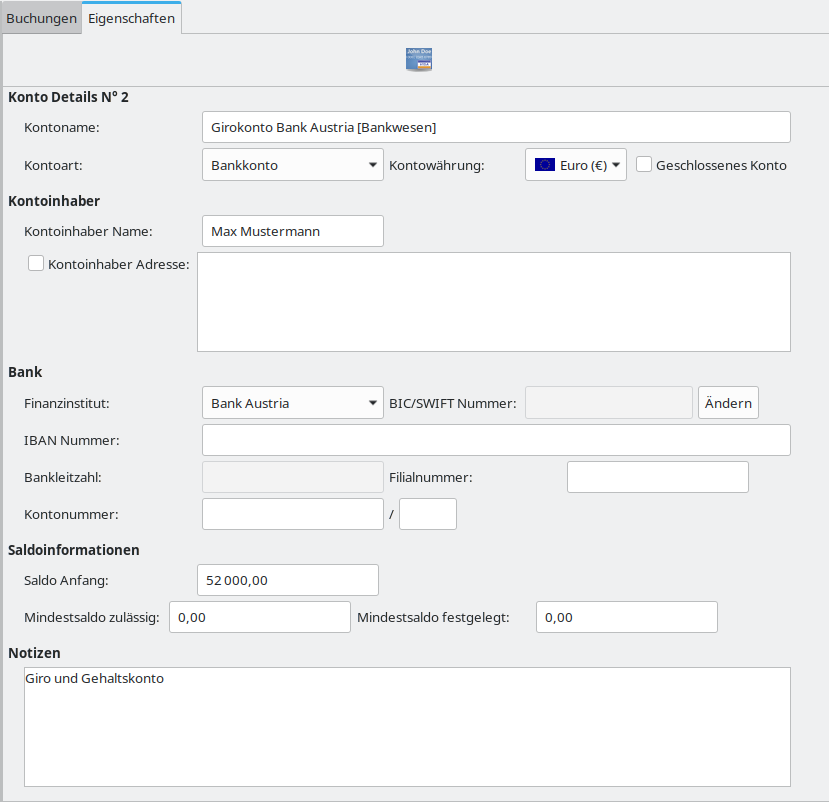
\includegraphics[width=0.95\textwidth]{image/screenshot/account_new_properties}
	\end{center}
	\caption{Konto \menus{Eigenschaften} Registerkarte}%Account \menus{Properties} tab}%Onglet \menus{Propriétés} d'un compte}
	\label{account-new-properties-img}
\end{figure}
% image centrée

Um die Eigenschaften eines Kontos anzuzeigen, wählen Sie es aus und klicken Sie dann im Bereich detail auf die Registerkarte \menus{Eigenschaften}. Auf dieser Registerkarte werden alle Informationen und Eigenschaften angezeigt, die bereits für das ausgewählte Konto eingegeben wurden.
%To view the properties of an account, select it and then click the \menus{Properties} tab in the details panel. This tab displays all the information and properties that have already been entered for the selected account.
%Pour afficher les propriétés d'un compte, sélectionnez-le, puis cliquez sur l'onglet \menus{Propriétés} dans le panneau des détails. Cet onglet affiche toutes les informations et propriétés qui ont déjà été renseignées sur le compte sélectionné\refimage{account-new-properties-img}.

Um diese Daten zu ändern, siehe Abschnitt \vref{accounts-modify}, \menus{Konto bearbeiten}.
%To modify this data, see the section \vref{accounts-modify}, \menus{Modify an account}.
%Pour modifier ces données, voir la section \vref{accounts-modify}, \menus{Modifier un compte}.

Die verschiedenen Informationen, die ein Konto enthalten kann, sind in fünf Abschnitte unterteilt:
%The various pieces of information that an account may contain are divided into five sections:
%Les différentes informations qu'un compte peut contenir sont divisées en cinq rubriques:

\begin{enumerate}
	\item \menus{Konto detail N° x}:
	%\menus{Account details No. x}:
	%\menus{Details du compte N°x}:
	\begin{itemize}
		\item \menus{Kontoname}: Dies kann ein beliebiger Name sein, zum Beispiel \emph{Girokonto}, \emph{Bankkonto 1} oder \emph{Bankkonto 2};
		%\menus{Account name}: this can be any name, for example \emph{Current account}, \emph{Bank account 1} or \emph{Bank account 2};
		%\menus{Nom du compte}: ce peut-être un nom quelconque, par exemple \emph{Compte courant}, \emph{Compte livret}, \emph{Compte banque 1} ou \emph{Compte banque 2};	
		% saut de ligne pour indentation correcte de la note dans la liste
		
		%\Note{}: dans le cas d'une comptabilité numérotée (association ou petite entreprise), les noms des comptes sont précédés du numéro fourni par le plan comptable, par exemple \enquote{512. Compte banque X }; ce libellé est donc une donnée alphanumérique.
		
		\item \menus{Kontoart}: Weitere Einzelheiten finden Sie im Abschnitt \vref{accounts-type};
		%\menus{Account type}: for more details, see section \vref{accounts-type};
		%\menus{Type du compte}: pour plus de détails, voir la section \vref{accounts-type};	
		\item \menus{Kontowährung}: die Währung, in der die Buchungen für dieses Konto abgewickelt werden (siehe Abschnitte \vref{setup-resources-currencies} und \vref{setup-resources-rate});
		%\menus{Account currency}: the currency in which transactions for this account are denominated (see sections \vref{setup-resources-currencies} and \vref{setup-resources-rate});
		%\menus{Devise du compte}: la devise dans laquelle les opérations de ce compte sont libellées (voir les sections \vref{setup-resources-currencies} et \vref{setup-resources-rate});	
		\item \menus{Geschlossenes Konto}\index{Konto!Geschlossenes}: Kontrollkästchen, mit dem Sie das Konto im Navigationsbereich und in der Informationsleiste ausblenden können, ohne es zu löschen; es kann durch Klicken auf das Menü \menus{Ansicht – Geschlossene Konten anzeigen} wieder eingeblendet werden;
		%\menus{Closed account}\index{account!closed}: checkbox that allows you to hide the account in the navigation panel and in the information bar, without deleting it; it can be displayed again by clicking on the \menus{View - Show closed accounts} menu;
		%\menus{{Compte clos}}\index{compte!clos}: case à cocher qui vous permet de masquer le compte dans le panneau de navigation et dans la barre d'information, sans pour autant le supprimer; il pourra être affiché à nouveau en cliquant sur le menu \menus{Affichage - Montrer les comptes clos};
	\end{itemize}
	\item \menus{Kontoinhaber}:
	%\menus{Account holder}:
	%\menus{Titulaire du compte}:
	\begin{itemize}
		\item \menus{Kontoinhaber Name}: Der Kontoinhaber kann für jedes Konto unterschiedlich sein, beispielsweise wenn Sie für jedes Ihrer Kinder ein Sparkonto eröffnen;
		%\menus{Account holder name}: the account holder may be different for each account, for example if you open a savings account for each of your children;
		%\menus{Nom du titulaire}: le titulaire d'un compte peut être différent pour chaque compte, par exemple si vous ouvrez un livret d'épargne pour chacun de vos enfants;	
		\item \menus{Address of the holder}: Der Inhaber kann dieselbe Adresse wie der Hauptinhaber haben oder eine andere Adresse, die hier nach Ankreuzen des Kästchens \menus{Eigene Adresse des Inhabers} anzugeben ist (siehe Absatz \vref{setup-display-addresses-address}, \menus{Adressen});
		%\menus{Address of the holder}: the holder may have the same address as the main holder, or a different address, which must be specified here after ticking the box \menus{Holder's own address} (see paragraph \vref{setup-display-addresses-address}, \menus{Addresses});
		%\menus{Adresse du titulaire}: le titulaire peut avoir la même adresse que le titulaire principal, ou bien une adresse différente qu'il faudra préciser ici après avoir coché la case \menus{Adresse du titulaire} (voir le paragraphe \vref{setup-display-addresses-address}, \menus{Adresses});
	\end{itemize}
	\item \menus{Bank}:
	%\menus{Banque}:
	\begin{itemize}
		\item \menus{Finanzinstitut}: die Bank, die Ihr Konto verwaltet; Sie können eine Bank aus der Dropdown-Liste auswählen oder auf \menus{Eine neue Bank erstellen} klicken; es ist ratsam, dieses Feld auszufüllen (siehe Abschnitt \vref{setup-resources-banks});
		%\menus{Financial institution}: the bank that manages your account; you can choose a bank from the drop-down list, or click on \menus{Add a new bank}; it is advisable to fill in this field (see section \vref{setup-resources-banks});
		%\menus{Établissement financier}: la banque qui gère votre compte; vous pouvez choisir une banque indiquée dans la liste déroulante, ou bien cliquer sur \menus{Ajouter une nouvelle banque}; il est conseillé de renseigner ce champ (voir la section \vref{setup-resources-banks});
		\item \menus{BIC/SWIFT Nummer}:Nachdem Sie eine vorhandene Bank ausgewählt haben, können Sie auf die Schaltfläche \menus{Ändern} klicken, um ein Fenster zum Bearbeiten der Bankeinstellungen zu öffnen;
		%\menus{BIC/SWIFT code}: after selecting an existing bank, you can click on the \menus{Modify} button to open a window for editing the bank's settings;
		%\menus{Code BIC}:	après avoir sélectionné une banque existante, vous pourrez cliquer sur le bouton \menus{Modifier} ouvrant une fenêtre pour éditer les paramètres de la banque;
		\item \menus{\gls{IBAN} nummer}: der Code, der auf Ihren Bankkontodaten oder der von der Bank bereitgestellten IBAN zu finden ist (siehe Abschnitt \vref{setup-resources-banks});
		%\menus{\gls{IBAN} number}: the code found on your bank account details (BBAN) or IBAN provided by the bank (see section \vref{setup-resources-banks});
		%\menus{N° \gls{IBAN}}: le code que vous trouverez sur votre relevé d'identité bancaire (RIB) ou IBAN fourni par la banque (voir la section \vref{setup-resources-banks});
		\item \menus{Bankleitzahl}: zeigt den Code des oben ausgewählten Finanzinstituts an;
		%\menus{Bank sort code}: displays the code of the financial institution selected above;
		%\menus{Code Banque}: affiche le code de l'établissement financier sélectionné au-dessus;	
		\item \menus{Filialnummer}: die Adresse Ihrer Bankfiliale, die Sie auch in Ihren Bankkontodaten finden (siehe Abschnitt \vref{setup-resources-banks});
		%\menus{Bank branch code}: the address of your bank branch, which can also be found on your bank account details (see the section \vref{setup-resources-banks});
		%\menus{Guichet/Agence}: l'adresse de votre agence bancaire, à relever également sur votre RIB (voir la section \vref{setup-resources-banks});	
		\item \menus{Kontonummer}: Ihre Bankdaten einsehen (siehe Abschnitt \vref{setup-resources-banks});
		%\menus{Account number / Key}: see your bank details (see section \vref{setup-resources-banks});
		%\menus{Numéro du compte/Clé}: voir sur votre RIB (voir la section \vref{setup-resources-banks});
	\end{itemize}
	\item \menus{Saldoinformationen}:
	%\menus{Balances}
	%\menus{Soldes}
	\begin{itemize}
		\item \menus{Saldo Anfang}: der Saldo Ihres letzten Kontoauszugs zum Zeitpunkt der Kontoeröffnung; es ist ratsam, den Eröffnungssaldo des Kontos auf Null zu belassen und dann eine erste Transaktion für den erforderlichen Betrag zu erstellen, da dies die zukünftige Abstimmung erleichtert; 
		%\menus{Initial balance}: the balance of your last bank statement at the time the account was created; it is advisable to leave the opening balance of the account at zero and then create an initial transaction for the required amount, as this will facilitate future reconciliation management;
		%\menus{Solde initial}: le solde de votre dernier relevé bancaire au moment de la création du compte; il est conseillé de laisser le solde initial du compte à zéro et de créer par la suite une opération initiale du montant nécessaire, car cela facilitera la gestion future des rapprochements;	
		\item \menus{Mindestsaldo zulässig}: der von Ihrem Finanzinstitut genehmigte Mindestsaldo, besser bekannt als Überziehungsrahmen;
		%\menus{Minimum authorised balance}: the minimum balance authorised by your financial institution, more commonly known as an overdraft facility;
		%\menus{Solde minimal autorisé}: le solde minimal que vous autorise votre établissement financier, plus communément appelé autorisation de découvert;	
		\item \menus{Mindestsaldo festgelegt}: Der Mindestsaldo, den Sie aufrechterhalten möchten; damit die Farbcodierung des Saldos auf der \menus{Startseite} ordnungsgemäß funktioniert, muss dieser größer oder gleich dem genehmigten Mindestsaldo sein.
		%\menus{Minimum desired balance}: the minimum balance you would like to maintain; for the balance colour coding on the \menus{Home} page to work properly, it must be greater than or equal to the minimum authorised balance;
		%\menus{Solde minimal voulu}: le solde minimal que vous aimeriez respecter; pour un bon fonctionnement de la mise en couleur des soldes dans la page \menus{Accueil}, il doit être supérieur ou égal au solde minimal autorisé;
	\end{itemize}	
	\item \menus{Notizen}: Eingabefeld für informelle Kommentare zum Konto: Eröffnungsdatum, Rendite usw. (siehe Abschnitt \vref{setup-resources-banks}).
	%\menus{Comments}: input field for informal comments on the account: opening date, rate of return, etc. (see section \vref{setup-resources-banks}).
	%\menus{Commentaires}: zone de saisie pour des commentaires informels sur le compte: date d'ouverture, taux de rendement, etc. (voir la section \vref{setup-resources-banks}).
\end{enumerate}

\section{Neues Konto erstellen\label{accounts-new}}%Creating a new account%Création d'un nouveau compte


\Note{}: Bevor Sie mit der Erstellung eines neuen Kontos beginnen, sollten Sie den Abschnitt \vref{accounts-type}, \menus{Kontoarten bei Grisbi} und den Abschnitt \vref{setup-resources-modes}, \menus{Zahlungsweisen} lesen, die ausführlichere Informationen zu den in Grisbi verfügbaren Optionen enthalten.
%\Note{}: before you start creating a new account, it is advisable to consult the section \vref{accounts-type}, \menus{Grisbi account types}, and the section \vref{setup-resources-modes}, \menus{Payment methods}, which provide much more detail about the options available in Grisbi.
%\Note{}: avant de commencer la création d'un nouveau compte, il est conseillé de consulter la section \vref{accounts-type}, \menus{Types de compte de Grisbi}, et la section \vref{setup-resources-modes}, \menus{Modes de règlement}, qui donnent beaucoup plus de détails sur les possibilités que Grisbi vous propose.
% espace après Attention ou Note: 5 mm
\vspacepdf{3mm}


%You can create a new account in two ways:
%Vous pouvez créer un nouveau compte de deux façons:
\begin{itemize}
	\item entweder durch Klicken auf das Menü \menus{Bearbeiten – Konto erstellen}\\
	(oder mit \keys{Strg+Shift+N});
	%either by clicking on the menu \menus{Edit - New Account} (or with \keys{Ctrl+Shift+N});
	%soit en cliquant sur le menu \menus{Éditer - Nouveau compte} (ou avec \keys{Ctrl+Maj+N});
	\item entweder durch einen Rechtsklick im Navigationsbereich, auf der Registerkarte \menus{Konten} oder auf einem bestehenden Konto und durch Klicken auf \menus{Konto erstellen} im Kontextmenü.
	%either by right-clicking in the navigation panel, on the \menus{Accounts} tab or on an existing account, and clicking \menus{New account} in the context menu.
	%soit en faisant un clic droit dans le panneau de navigation, sur l'onglet \menus{Comptes} ou sur un compte existant et en cliquant sur \menus{Nouveau compte} dans le menu contextuel.
\end{itemize}
Der Assistent \menus{Ein neues Konto erstellen}, bestehend aus vier Schritten, wird geöffnet:
%The \menus{Create a new account} wizard, consisting of four steps, opens:
%L'assistant \menus{Créer un nouveau compte} comprenant quatre étapes, s'ouvre:
\begin{enumerate}
	\item Begrüßungsbildschirm (Schritt 1/4); bestätigen Sie durch Klicken auf die Schaltfläche \menus{Weiter};
	%welcome screen (step 1/4); confirm by clicking the \menus{Next} button;
	%accueil de l'assistant (étape 1/4); validez par le bouton \menus{Suivant};
	\item \menus{Kontoart Auswahl}\refimage{account-new-type-img} (Schritt 2/4):
	%\menus{Select account type}\refimage{account-new-type-img} (step 2/4):
	%\menus{Sélection du type de compte}\refimage{account-new-type-img} (étape 2/4): 
	\begin{figure}[htbp]
		\begin{center}
			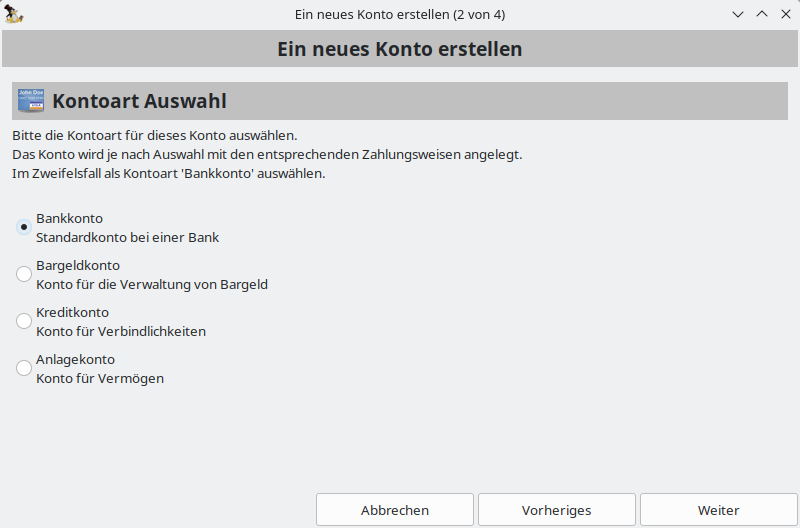
\includegraphics[width=0.95\textwidth]{image/screenshot/account_new_type}
		\end{center}
		\caption{Choice of new account type}%Choix du type du nouveau compte}
		\label{account-new-type-img}
	\end{figure}
	
	Wählen Sie aus den vier verfügbaren Kontotypen aus und bestätigen Sie Ihre Auswahl, indem Sie auf die Schaltfläche \menus{Weiter} klicken;
	%Choose from the four types of accounts available, then confirm by clicking the \menus{Next} button.
	%Faites votre choix parmi les quatre types de compte proposés, puis validez par le bouton \menus{Suivant};
	% espace pour Note ou Attention à la ligne dans une liste
	
	%\vspacepdf{3mm}
	\Note{}: Achten Sie bei der Erstellung eines neuen Kontos darauf, den richtigen Kontoart auszuwählen, da Sie sonst später möglicherweise alle darin erfassten Transaktionen auf ein neues, besser geeignetes Konto übertragen müssen.
	%\Note{}: when creating a new account, be careful to choose the correct account type, otherwise you may later have to transfer all the transactions you have entered into it to a new, more appropriate account.
	%\Note{}: lorsque vous créez un nouveau compte, faites attention à choisir un type de compte correct, sinon vous pourriez être amené, plus tard, à transférer toutes les opérations que vous y auriez saisies dans un nouveau compte plus adéquat.
	
	\item Im folgenden Fenster können Sie dieses neue Konto konfigurieren \refimage{account-new-creation-img}:
	%the following window allows you to configure this new account \refimage{account-new-creation-img}:
	%la fenêtre suivante vous permet de paramétrer ce nouveau compte \refimage{account-new-creation-img}:
	% image centrée
	\begin{figure}[htbp]
		\begin{center}
			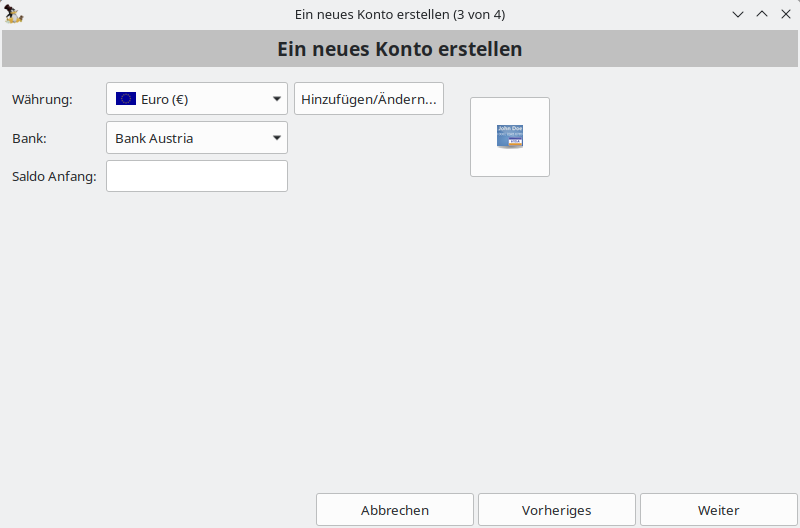
\includegraphics[width=0.95\textwidth]{image/screenshot/account_new_currency}
		\end{center}
		\caption{Neue Kontoeinstellungen}%New account settings}%Paramètres du nouveau compte}
		\label{account-new-creation-img}
	\end{figure}
	% image centrée
		\begin{enumerate}
			\item Wählen Sie die Kontowährung aus der Dropdown-Liste aus, die die Ihrer Grisbi-Datei bereits bekannten Währungen enthält. Andernfalls klicken Sie auf \menus{Hinzufügen/Ändern...}, woraufhin ein Fenster mit einer Dropdown-Liste erscheint, die alle Grisbi bekannten Währungen enthält. Die Details der ausgewählten Währung werden unten in Feldern angezeigt, die Sie noch ändern können. Bestätigen Sie anschließend mit einem Klick auf die Schaltfläche \menus{Schließen},
			%select the account currency from the drop-down list, which contains the currencies already known to your Grisbi file; otherwise, click on \menus{Add/Change...}, and a window will appear with a drop-down list containing all the currencies known to Grisbi; the details of the selected currency are displayed below, in fields that you can still modify; then confirm by clicking on the \menus{Close} button.
			%choisissez la \indexword{devise}\index{devise} du compte dans la liste déroulante, qui propose les devises que connaît déjà votre fichier Grisbi; sinon, cliquez sur \menus{Ajouter/Changer}, une fenêtre s'affiche, où une liste déroulante vous propose toutes les devises du monde connues par Grisbi; les détails de la devise sélectionnée s'affichent en-dessous, dans des champs que vous pouvez encore modifier; puis validez par le bouton \menus{Fermer},
			\item Wählen Sie die \indexword{Bank}\index{Bank!Erstellung}, die dieses Konto führt, aus der Dropdown-Liste aus, in der die Ihrer Grisbi-Datei bereits bekannten Banken angezeigt werden; Andernfalls klicken Sie auf \menus{Eien neue Bank erstellen}: Es erscheint ein Fenster, in dem Sie den Namen der Bank und viele weitere Details eingeben können. Bestätigen Sie anschließend mit einem Klick auf die Schaltfläche {Anwenden},
			%select the \indexword{bank}\index{bank!creation} that holds this account from the drop-down list, which shows the banks already known to your Grisbi file; otherwise, click on \menus{Add new bank}: a window will appear where you can enter the name of the bank and many other details; then confirm by clicking on the \menus{Apply} button.
			%choisissez la \indexword{banque}\index{banque!création} qui détient ce compte dans la liste déroulante et qui propose les banques que connaît déjà votre fichier Grisbi; sinon, cliquez sur \menus{Ajouter une nouvelle banque}: une fenêtre s'affiche, où vous pouvez renseigner le nom de la banque et de nombreux autres détails; puis validez par le bouton \menus{Fermer},
			\item Geben Sie den Saldo Anfang ein,
			%\item enter the opening balance,
			%\item saisissez le solde initial,

			\Note{}: Es ist ratsam, den Saldo Anfang auf Null zu belassen und gegebenenfalls nachträglich eine Buchung Anfang über den erforderlichen Betrag zu erstellen, da dies die zukünftige Abstimmung erleichtert.
			%\Note{}: it is advisable to leave the initial account balance at zero and, if necessary, to subsequently create an initial transaction for the required amount, as this will facilitate future reconciliation management.
			%\Note{}: il est conseillé de laisser le solde initial du compte à zéro et, si besoin est, de créer par la suite une opération initiale du montant nécessaire, car cela facilitera la gestion future des rapprochements.
			
			\item Wählen Sie das \indexword{Icon}\index{Icon} für das Konto aus, indem Sie darauf klicken: Es erscheint ein Fenster, in dem Sie entweder ein Verzeichnis aus der Dropdown-Liste auswählen und dann auf eines der Icon darunter klicken oder im Dateisystem Ihres Computers nach einer Datei suchen können (über die Schaltfläche \menus{Durchsuchen}). Wenn Sie Ihr Icon gefunden haben, bestätigen Sie Ihre Auswahl, indem Sie auf die Schaltfläche \menus{Prüfen} klicken,
			%\item select the \indexword{icon}\index{icon} for the account by clicking on it: a window will appear where you can either select a directory from the drop-down list and then click on one of the icons below, or search for a file in your computer's file system (using the \menus{Browse} button). once you have found your icon, confirm by clicking on the \menus{Validate} button,
			%\item choisissez l'\indexword{icône}\index{icône} du compte en cliquant dessus: une fenêtre s'affiche, où vous pouvez soit choisir un répertoire dans la liste déroulante puis cliquer sur une des icônes en-dessous, soit chercher un fichier dans le système de fichiers de votre ordinateur (bouton \menus{Parcourir}); une fois votre icône trouvée, validez par le bouton \menus{Valider},
			\item Bestätigen Sie anschließend Ihre Einstellungen, indem Sie auf die Schaltfläche \menus{Weiter} klicken.
			%\item then confirm your settings by clicking on the \menus{Next} button.
			%\item puis validez vos paramètres en cliquant sur le bouton \menus{Suivant}.
		\end{enumerate}
	\item Im letzten Fenster\refimage{account-new-name-img} können Sie den Namen des neuen Kontos eingeben, der im Navigationsbereich angezeigt wird. Bestätigen Sie anschließend durch Klicken auf die Schaltfläche \menus{Schließen}.
	%\item the last window\refimage{account-new-name-img} allows you to enter the name of the new account, which will appear in the navigation panel; then confirm by clicking the \menus{Close} button.
	%la dernière fenêtre\refimage{account-new-name-img} vous permet de saisir le nom du nouveau compte, celui qui apparaîtra dans le panneau de navigation; puis validez par le bouton \menus{Fermer};
	% image centrée
	\begin{figure}[htbp]
		\begin{center}
			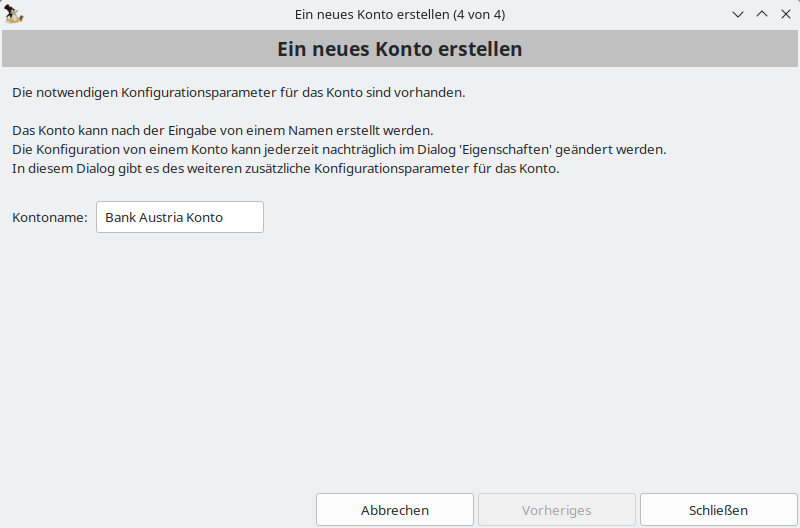
\includegraphics[width=0.95\textwidth]{image/screenshot/account_new_name}
		\end{center}
		\caption{Eingabe des Namens des neuen Kontos}%Entering the name of the new account}%Saisie du nom du nouveau compte}
		\label{account-new-name-img}
	\end{figure}
	% image centrée
	\item Das neue Konto wird dann erstellt und im Navigationsbereich ausgewählt: Sein Name erscheint auf einem \colorbox[RGB]{235,149,149}{dunkelrosa Hintergrund}, und im Bereich details wird die Registerkarte \menus{Eigenschaften} angezeigt, auf der Sie die Einstellungen ändern oder vervollständigen können; die Registerkarte \menus{Buchungen} enthält natürlich noch keine Buchungen.
	%\item the new account is then created and selected in the navigation panel: its name appears on a \colorbox[RGB]{235,149,149}{dark pink background}, and the details panel displays the \menus{Properties} tab, where you can modify or complete the settings; the \menus{Operations} tab is, of course, empty of any operations.
	%le nouveau compte est alors créé et sélectionné dans le panneau de navigation: son nom apparaît sur \colorbox[RGB]{235,149,149}{fond rose foncé}, le panneau des détails affiche l'onglet \menus{Propriétés} où vous pourrez modifier ou compléter les paramètres; l'onglet \menus{Opérations} est bien sûr vide de toute opération.
\end{enumerate}

%espace pour changement de thème
\vspacepdf{3mm}
Nur wenn Sie Ihre Grisbi-Datei unmittelbar vor der Erstellung dieses Kontos angelegt haben, kehren Sie zum Ende des Abschnitts \vref{start-newfile-end}, \menus{Erstellen einer neuen Kontodatei}, zurück. Gehen Sie zu dem Absatz, der mit \emph{Auf die eine oder andere Weise\ldots{}} beginnt und Sie auffordert, sofort weitere Konten anzulegen.
%If, and only if, you have just created your Grisbi file immediately prior to creating this account, return to the end of the section \vref{start-newfile-end}, \menus{Creating a new account file}. Go to the paragraph beginning with \emph{One way or another\ldots{ }}, which will prompt you to create other accounts immediately.
%Si, et seulement si vous venez de créer votre fichier Grisbi juste avant cette création de compte, revenez à la fin de la section \vref{start-newfile-end}, \menus{Création d'un nouveau fichier de comptes}. Allez juste après la fin de la procédure de création du fichier de comptes, au paragraphe commençant par \emph{D'une manière ou d'une autre\ldots{ }}, ce qui vous proposera de créer tout de suite d'autres comptes.

%espace pour changement de thème
\vspacepdf{5mm}
Andernfalls können Sie das soeben erstellte Konto verwenden.
%Otherwise, you can start using the account you just created.
%Sinon, vous pouvez commencer à utiliser le compte que vous venez de créer.

%espace pour changement de thème
\vspacepdf{5mm}
Sie können die Zahlungsmethoden für dieses Konto auch im Menü \menus{Bearbeiten – Einstellungen} detailliert konfigurieren (siehe Abschnitt \vref{setup-resources-modes}, \menus{Zahlungsweizen}).
%You can also configure the payment methods for this account in detail in the \menus{Edit - Preferences} menu (see the \vref{setup-resources-modes} section, \menus{Payment methods}).
%Vous pouvez aussi configurer précisément les modes de règlement des opérations de ce compte dans le menu \menus{Éditer - Préférences} (voir la section \vref{setup-resources-modes}, \menus{Modes de règlement}).


\section{Konto bearbeiten\label{accounts-modify}}%Editing an account%Modification d'un compte

Um ein Konto zu bearbeiten, wählen Sie das Konto im Navigationsbereich oder über die Informationsleiste aus und klicken Sie dann im Bereich Details auf die Registerkarte \menus{Eigenschaften}\refimage{account-new-properties-img}.
%To edit an account, select the account in the navigation panel or using the information bar, then click the \menus{Properties}\refimage{account-new-properties-img} tab in the details panel.
%Pour modifier un compte, sélectionnez le compte dans le panneau de navigation ou avec la barre d'information, puis cliquez sur l'onglet \menus{Propriétés}\refimage{account-new-properties-img} dans le panneau des détails.

Die folgenden Felder müssen ausgefüllt werden:
%The following fields must be completed:
%Les champs suivants doivent obligatoirement être renseignés:
\begin{itemize}
	\item Abschnitt \menus{Konto Details N° x}:
	%\item section \menus{Account details No. x}:
	%rubrique \menus{Détails du compte N°x}:
	\begin{itemize}
		\item der \menus{Kontoname};
		%\item the \menus{Account name};
		%le \menus{Nom du compte};
		\item der \menus{Kontoart};
		%\item the \menus{Account type};
		%le \menus{Type du compte};
		\item der \menus{Kontowährung};
		%\item the \menus{Account currency};
		%la \menus{Devise du compte};
	\end{itemize}
	\item Abschnitt \menus{Saldoinformationen}:
	%\item section \menus{Balances}:
	%rubrique \menus{Soldes}:
	\begin{itemize}
		\item der \menus{Saldo Anfang}.
		%\item the \menus{Initial balance}.
		%le \menus{Solde initial}.
	\end{itemize}
\end{itemize}
Alle anderen Felder sind optional.
%All other fields are optional.
%Tous les autres champs sont facultatifs. 

Sie können \emph{alle} diese Informationen jederzeit ändern.
%You can change \emph{all} of this information at any time.
%Vous pourrez modifier à tout moment \emph{toutes} ces informations.

Die Felder \menus{Kontoart}, \menus{Kontowährung} und \menus{Finanzinstitut} bieten Zugriff auf eine Dropdown-Liste, die zum Ausfüllen des Feldes verwendet werden kann.
%The fields \menus{Account type}, \menus{Account currency}, \menus{Financial institution} provide access to a drop-down list that can be used to fill in the field.
%Les champs \menus{Type du compte}, \menus{Devise du compte}, \menus{Établissement financier} donnent accès à une liste déroulante permettant de renseigner le champ.

Die weißen Textfelder (im Gegensatz zu den grauen Feldern) können über die Tastatur ausgefüllt werden. Über ein Kontextmenü, das durch einen Rechtsklick in einem Eingabefeld aufgerufen wird, können Sie folgende Aktionen ausführen:
%The white text fields (as opposed to the grey fields) can be filled in using the keyboard, and a context menu accessible by right-clicking in an input field allows you to perform the following actions:
%Les champs blancs de texte (à l'opposé des champs gris) peuvent être remplis au clavier, et un menu contextuel accessible par un clic-droit dans un champ de saisie permet d'effectuer les actions suivantes:
\begin{itemize}
	\item \menus{Ausschneiden} (die Auswahl);
	%\item \menus{Cut} (the selection);
	%\menus{Couper} (la sélection);
	\item \menus{Copieren} (die Auswahl);
	%\item \menus{Copy} (the selection);
	%\menus{Copier} (la sélection);
	\item \menus{Einfügen} (die Auswahl);
	%\item \menus{Paste} (the selection);
	%\menus{Coller} (la sélection);
	\item \menus{Löschen} (die Auswahl);
	%\item \menus{Delete} (the selection);
	%\menus{Supprimer} (la sélection);
	\item \menus{Alles auswählen} in das dafür vorgesehene Feld;
	%\item \menus{Select all} in the field provided;
	%\menus{Tout sélectionner} dans le champ renseigné;
	\item \menus{Emoji einfügen}\index{emoji}: öffnet ein Fenster, über das Sie auf alle Arten von Emoticons und Symbolen zugreifen können.
	%\item \menus{Insert emoji}\index{emoji}: opens a window giving access to all kinds of emoticons and icons.
	%\menus{Insérer un émoji}\index{émoji}: ouvre une fenêtre donnant accès à toutes sortes d'émoticônes et d'icônes.
\end{itemize}


% espace avant Attention ou Note: 5 mm
\vspacepdf{3mm}
\Attention{}: Wenn Sie bestimmte Eigenschaften wie den Kontotyp ändern, müssen Sie alle bereits eingegebenen Vorgänge \emph{einzeln} an die neuen Kontoeigenschaften anpassen. In jedem Fall \textbf{müssen} Sie vor jeder Änderung an den Konten eine Sicherungskopie Ihrer Kontodatei erstellen.
%If you change certain properties such as the account type, you will need to adapt all operations already entered to the new account properties \emph{individually}. In any case, before making any changes to the accounts, you \textbf{must} back up your account file.
%\Attention{}: si vous modifiez certaines propriétés comme le type du compte, cela nécessitera d'adapter, \emph{individuellement}, toutes les opérations déjà saisies aux nouvelles propriétés du compte. Dans tous les cas, avant de procéder à une quelconque modification des comptes, faites \textbf{impérativement} une sauvegarde de votre fichier de comptes.

% saut de page pour titre solidaire
\section{Konto schließen\label{accounts-closure}}%Closing an account%Clôture d'un compte

Auf diese Weise können Sie ein Konto ausblenden, ohne es zu löschen (siehe Vorgehensweise unter \menus{Kontodaten}\vref{accounts-properties}, Absatz {1. Konto detail N° x}, Option {Geschlossenes Konto}).
%This allows you to hide an account without deleting it (see the procedure in the \menus{Account properties}\vref{accounts-properties}, paragraph \menus{1. Account details No. x}, option \menus{Closed account}).
%Cela vous permet de masquer un compte sans le supprimer (voir la procédure dans les \menus{Propriétés d'un compte} \vref{accounts-properties}, paragraphe \menus{1. Détails du compte N°x}, option \menus{Compte clos}).


\section{Konto löschen\label{accounts-delete}}%Deleting an account%Suppression d'un compte

Es gibt zwei Möglichkeiten, ein Konto zu löschen:
%There are two ways to delete an account:
%Vous pouvez supprimer un compte de deux façons:
\begin{itemize}
	\item entweder durch Auswahl eines Kontos, wobei die Registerkarte \menus{Buchungen} im Bereich details angezeigt wird, und anschließendes Klicken auf das Menü \menus{Bearbeiten – Konto löschen} in der Menüleiste,
	%either by selecting an account, with the \menus{Operations} tab displayed in the details panel, then clicking on the \menus{Edit - Remove current account} menu in the menu bar,
	%soit en sélectionnant un compte, avec l'onglet \menus{Opérations} affiché dans le panneau des détails, puis en cliquant sur le menu \menus{Éditer - Supprimer le compte courant} de la barre de menu,
	\item entweder durch einen Rechtsklick auf ein Konto im Navigationsbereich, wodurch ein Kontextmenü geöffnet wird, über das Sie auf die Option \menus{Konto löschen} zugreifen können.
	%either by right-clicking on an account in the navigation panel, which opens a context menu giving access to the \menus{Remove this account} option.
	%soit par un clic droit sur un compte dans le panneau de navigation qui ouvre un menu contextuel donnant accès à l'option \menus{Supprimer ce compte}.
\end{itemize}

Es öffnet sich ein Bestätigungsdialogfeld. Wenn Sie den Löschvorgang bestätigen möchten, klicken Sie auf die Schaltfläche \menus{Ja}.
%A confirmation dialogue box will open; if this is what you want, confirm the deletion by clicking the \menus{Yes} button.
%Une boîte de dialogue de confirmation s'ouvre; si c'est vraiment ce que vous voulez, validez la suppression avec le bouton \menus{Oui}.
% espace avant Attention ou Note: 5 mm

\vspacepdf{3mm}
\Attention{}: Es wird keine weitere Warnung erfolgen, und das Konto wird zusammen mit allen Transaktionen gelöscht. Diese Maßnahme ist \indexword{\textbf{unumkehrbar}}\index{Maßnahme!unumkehrbar}!
%there will be no further warning, and the account, along with all its transactions, will be deleted. This action is \indexword{\textbf{irreversible}}\index{action!irréversible}!
%\Attention{}: il n'y aura pas d'autre avertissement, et le compte, ainsi que toutes ses opérations, sera supprimé. Cette action est \indexword{\textbf{irreversible}}\index{action!irreversible}!
\newline

\noindent
\underline{\textbf{Anmerkung des Übersetzers}}: Die folgenden Abschnitte sind die Übersetzung des französischen Handbuchs und keine Übertragung auf das deutsche Rechnungswesen. Darüber hinaus verfügt der Autor nicht über die erforderlichen Sprach- und Buchhaltungskenntnisse in Deutsch. Daher kann die Richtigkeit der Beispiele und der verwendeten Begriffe nicht garantiert werden.
\newline
Ein Korrektor wäre sehr willkommen.
%Note de traduction: les sections suivantes sont la traduction du manuel français et non la transposition vers la comptabilité allemande. De plus, l'auteur n'a pas les compétences linguistiques et comptables allemandes. Donc l'exactitude des exemples et des termes employés n'est pas garantie.
%Un/une correcteur-trice sera le/la bienvenu-e.


\section{Arten von Grisbi-Konten\label{accounts-type}}%Types of Grisbi accounts%Types de compte de Grisbi

Wie zu Beginn dieses Kapitels erwähnt, kann Grisbi vier \indexword{Arten von Konten}\index{Arten von Konten} verwalten:
%As stated at the beginning of this chapter, Grisbi can manage four \indexword{types of accounts}\index{types of accounts}:
%Comme énoncé en début de chapitre, Grisbi sait gérer quatre \indexword{types de compte}\index{types de compte}:

\begin{itemize}
	\item Bankkonto: Es ermöglicht Ihnen, jede Art von Buchhaltungsvorgang durchzuführen (siehe \vref{accounts-type-bank});
	%bank account: it allows you to perform all types of transactions (see \vref{accounts-type-bank});
	%compte bancaire: il permet de faire tout type d'opération (voir \vref{accounts-type-bank});
	\item Bargeldkonto: Es ermöglicht Ihnen lediglich die Verwaltung von Bargeld (siehe \vref{accounts-type-cash});
	%cash account: it only allows you to manage cash (see \vref{accounts-type-cash});
	%compte de caisse: il ne permet de gérer que des espèces (voir \vref{accounts-type-cash});
	\item Kreditkonto: Es ermöglicht Ihnen, eine Schuld zu verwalten, die Sie zurückzahlen (siehe \vref{accounts-type-liabilities});
	%liability account: this allows you to manage a debt that you are repaying (see \vref{accounts-type-liabilities});
	%compte de passif: il permet de gérer une dette que vous remboursez (voir \vref{accounts-type-liabilities}); 
	\item Anlagekonto: Es ermöglicht Ihnen die Verwaltung eines Vermögenswerts, der im Laufe der Zeit an Wert verliert (siehe \vref{accounts-type-assets}).
	%asset account: this allows you to manage an asset that depreciates over time (see \vref{accounts-type-assets}).
	%compte d'actif: il permet de gérer un bien qui se déprécie avec le temps (voir \vref{accounts-type-assets}).
\end{itemize}

%espace pour changement de thème
\vspacepdf{3mm}
In diesem Abschnitt werden die Funktionen und die Verwendung der einzelnen Kontotypen beschrieben.
%This section describes the features and usage of each of these account types.
%Cette section décrit les fonctionnalités et l'utilisation de chacun de ces types de compte.


\subsection{Typ \emph{Bankkonto}\label{accounts-type-bank}}%Type \emph{bank account}%Type \emph{compte bancaire}

Der Kontotyp \emph{Bankkonto} erlaubt alle Arten von Transaktionen, egal ob Soll oder Haben. Daher muss er für alle folgenden Konten verwendet werden:
%The account type \emph{bank account} allows all types of transactions, whether debit or credit. Therefore, it must be used for all of the following accounts:
%Le type de compte \emph{compte bancaire} admet tous les types d'opérations, en débit ou en crédit. De ce fait, il doit être utilisé pour tous les comptes suivants:
\begin{itemize}
	\item Bankkonto oder Girokonto;
	%bank account or current account;
	%compte bancaire ou compte courant;
	\item Sparkonto;
	%savings account;
	%compte d'épargne;
	\item Konto für \indexword{Debit-Bankkarte}\index{Bankkarte!Debit};
	%account for \indexword{debit bank card}\index{card!debit};
	%compte de \indexword{carte bancaire à débit immédiat}\index{carte bancaire!débit immédiat};
	\item \indexword{Kreditkartenkonto}\index{Kreditkartenkonto};
	%\indexword{credit card}\index{card!credit} account;
	%compte de \indexword{carte de crédit}\index{carte bancaire!de crédit};		
	\item Zwischenkonto;
	%suspense account;
	%compte d'attente;
	\item Vorschusskonto.
	%advance account.
	%compte d'avances. 
\end{itemize}

In den folgenden Abschnitten werden diese Konten beschrieben, die den Kontotyp \emph{Bankkonto} verwenden müssen.
%The following paragraphs describe these accounts, which must use the account type \emph{bank account}.
%Les paragraphes suivants décrivent ces comptes qui doivent utiliser le type de compte \emph{compte bancaire}.


\subsubsection{Bankkonto, Girokonto, Sparkonto oder Debitkartenkonto\label{accounts-type-bank-misc}}
	%Bank account, current account, savings account or debit card account
	%Compte bancaire, courant, d'épargne ou de carte bancaire à débit immédiat\label{accounts-type-bank-misc}}

Diese Konten dienen zur Erfassung aller Transaktionen, die Sie mit Ihrer Bank durchführen können:
%These accounts are used to record all the transactions you can carry out with your bank:
%Ces comptes servent à enregistrer toutes les opérations que vous pouvez faire avec votre banque: 

\begin{itemize}
	\item Überweisung von Konto zu Konto;
	%account-to-account transfer;
	%virement de compte à compte;
	\item Abbuchung vom Konto;
	%debit from the account;
	%prélèvement sur le compte;
	\item Ausstellen und Einreichen von Schecks;
	%issuing and depositing cheques;
	%émission et dépôt de chèques; 
	\item Kauf, Rückerstattung, Abhebung und Einzahlung mit einer \indexword{Debitkarte}\index{Debitkarte}.
	%purchase, refund, withdrawal and deposit with an \indexword{debit bank card}\index{card!debit}.
	%achat, remboursement, retrait et dépôt avec une \indexword{carte bancaire à débit immédiat}\index{carte bancaire!débit immédiat}. 
\end{itemize}


\subsubsection{Kreditkartenkonto\label{accounts-type-bank-creditcard}}
	%Credit card account\label{accounts-type-bank-creditcard}}
	%Compte de carte de crédit\label{accounts-type-bank-creditcard}}

Ein Kreditkartenkonto ist ein Bankkartenkonto, auf das sowohl Lastschriften als auch Gutschriften in Form von Überweisungen oder Darlehen (z. B. revolvierender Kredit) eingehen können. Sein Saldo kann daher positiv oder negativ sein.
%A credit card account is a bank card account that can receive debits as well as credits, either in the form of transfers or loans (e.g. revolving credit). Its balance can therefore be positive or negative.
%Un compte de carte de crédit est un compte de carte bancaire qui peut recevoir du débit, mais aussi du crédit, soit sous forme de virement, soit sous forme de prêt (par ex. un crédit renouvelable). Son solde peut donc être positif ou négatif.


\subsubsection{Zwischenkonto\label{accounts-type-bank-waiting}}
	%Suspense account\label{accounts-type-bank-waiting}}
	%Compte d'attente\label{accounts-type-bank-waiting}}

Ein Zwischenkonto dient zur Erfassung von Transaktionen (in der Regel Einnahmen), die noch auf die Überweisung auf ein Bank- oder Bargeldkonto warten. Es wird normalerweise bis zur Überweisung auf das Bank- oder Bargeldkonto gutgeschrieben, wodurch es wieder einen Saldo von Null aufweist.
%A suspense account is used to record transactions (usually receipts) pending transfer to a bank or cash account. It is normally credited until the transfer to the bank or cash account, which brings it back to a zero balance.
%Un compte d'attente sert à enregistrer des opérations (normalement des recettes) en attendant de les virer vers un compte bancaire ou de caisse. Il est normalement créditeur, jusqu'au moment du virement vers le compte bancaire ou de caisse, qui le ramène à un solde nul.

Die \indexword{Einzahlung von Schecks}\index{Einzahlung!Schecks} und die \indexword{Einzahlung von Bargeld}\index{Einzahlung!Bargeld} sind typische Beispiele für die Nützlichkeit des Zwischenkontos.
%The \indexword{deposit of cheques}\index{deposit!cheques} and the \indexword{deposit of cash}\index{deposit!cash} are typical examples of the usefulness of the suspense account.
%La \indexword{remise de chèques}\index{remise!chèques} et la \indexword{remise d'espèces}\index{remise!espèces} sont des exemples-type de l'utilité du compte d'attente. 

\paragraph{\textsl{Lieferung von Schecks oder Bargeld:}\label{accounts-type-bank-waiting-remittance}}
	%\textsl{Delivery of cheques or cash:}\label{accounts-type-bank-waiting-remittance}
	%\textsl{Remise de chèques ou d'espèces:}\label{accounts-type-bank-waiting-remittance}

Wenn Sie nur wenige Schecks oder Bargeld erhalten, ist es am einfachsten, diese direkt in Ihr Bankkonto (oder Bargeldkonto) einzutragen. In diesem Fall lesen Sie bitte den Abschnitt \vref{transactions-new-cheque}, \menus{Einzahlung von Schecks oder Bargeld}.
%If you receive few cheques or cash, the simplest thing to do is to enter them directly into your bank account (or cash account). In this case, refer to the section \vref{transactions-new-cheque}, \menus{Depositing cheques or cash}.
%Si vous recevez peu de chèques ou d'espèces, le plus simple est de les saisir directement dans votre compte bancaire (ou dans votre compte de caisse). Dans ce cas, reportez-vous à la section \vref{transactions-new-cheque}, \menus{Remise de chèques ou d'espèces}.

% espace pour changement de thème
\vspacepdf{3mm}
Wenn Sie jedoch eine große Anzahl von Schecks erhalten (z. B. weil Sie einen Verein verwalten und Ihre Mitglieder ihre Mitgliedsbeiträge per Scheck bezahlen), ist die effizienteste Lösung die Verwendung eines Zwischenkontos.
%However, if you receive a large number of cheques (for example, because you manage an association and your members pay their membership fees by cheque), the most efficient solution is to use a suspense account.
%Mais si vous recevez beaucoup de chèques (par exemple parce que vous gérez une association et que vos adhérents payent leur cotisation par chèque), le plus efficace est d'utiliser un compte d'attente.

% espace pour changement de thème
\vspacepdf{3mm}
Die Methode besteht daher darin, ein \emph{Zwischenkonto} anzulegen, das Sie beispielsweise \emph{Einzulösende Schecks} nennen könnten. Wenn Sie Schecks erhalten, verbuchen Sie diese einzeln in diesem Konto, wobei jeder Scheck einem \menus{Empfänger} entspricht. Wenn Sie die Schecks bei der Bank einreichen, tätigen Sie eine Überweisung von diesem Konto \emph{Einzulösende Schecks} auf Ihr Bankkonto in Höhe des Gesamtbetrags dieser Schecks, d. h. des Saldos des Kontos \emph{Einzulösende Schecks}. Erstellen Sie einen Zahlungsempfänger mit dem Namen \emph{Scheckeinzahlung}, wählen Sie \menus{Zahlung} als \menus{Zahlungsweisen} und geben Sie die Nummer Ihres Einzahlungsbelegs in das Feld \menus{Schecknummer} ein.
%The method therefore consists of creating a \emph{suspense account}, which you could name, for example, \emph{Cheques to be cashed}. As you receive cheques, you record them individually in this account, with each cheque corresponding to a \menus{Payee}. When you deposit the cheques at the bank, you make a transfer from this \emph{Cheques to be cashed} account to your bank account for the total amount of these cheques, i.e. the balance of the \emph{Cheques to be cashed} account. Create a payee called \emph{Cheque Deposit}, select \menus{Transfer} as the \menus{method of payment} and enter the number of your deposit slip in the \menus{Cheque/Transfer Number} field.
%La méthode consiste donc à créer un \emph{compte d'attente}, que vous nommez par exemple \emph{Chèques à encaisser}. Au fur et à mesure de la réception des chèques, vous les enregistrez individuellement dans ce compte, dont chaque chèque correspond à un \menus{Tiers}. Quand vous déposez les chèques à la banque, vous faites un virement de ce compte \emph{Chèques à encaisser} vers votre compte bancaire, du montant de l'ensemble de ces chèques, donc du solde du compte \emph{Chèques à encaisser}. Créez pour l'occasion un tiers \emph{Remise de chèques}, sélectionnez \menus{Virement} comme \menus{choix du mode de règlement} et dans le champ \menus{N° Chèque/Virement}, saisissez le numéro de votre bordereau de remise.
% (ce bordereau sera généré directement par Grisbi dans une prochaine version). 

Der Saldo des Kontos \emph{Einzulösende Schecks} wird dann auf Null zurückgesetzt, und der Betrag der Einzahlung wird dem Bankkonto gutgeschrieben, genau so, wie er auf Ihrem Kontoauszug erscheint. Auf diese Weise können Sie sowohl die Informationen von Dritten zu jedem Scheck als auch die gesamten Einzahlungsinformationen nachverfolgen.
%The balance of the \emph{Cheques to be cashed} account is then reset to zero, and the bank account is credited with the amount of the deposit, exactly as it will appear on your bank statement. This allows you to keep track of both the third-party information for each cheque and the overall deposit information.
%Le solde du compte \emph{Chèques à encaisser} revient alors à zéro, et le compte bancaire est crédité du montant de la remise, exactement comme le sera votre relevé bancaire. Ainsi vous gardez et l'information du tiers pour chaque chèque, et celle de la remise globale.

Anschließend führen Sie eine Pseudo-Abstimmung des Kontos \emph{Einzulösende Schecks} durch, indem Sie einen Nullsaldo vor dem Eingang des nächsten Schecks simulieren: Überprüfen Sie, ob diese Abstimmung eine Nummer hat, oder vergeben Sie eine Nummer, z. B. ÜBE-01, damit Sie später feststellen können, welcher Scheck zu welcher Einzahlung gehörte.
%You then perform a pseudo-reconciliation of the \emph{Cheques to be cashed} account by simulating a zero balance statement before the next cheque is received: check that this reconciliation has a number, or give it one, for example DEP-01, which will allow you to later find which cheque was part of which deposit.
%Vous faites ensuite un pseudo-rapprochement du compte \emph{Chèques à encaisser} en simulant un relevé de solde nul avant la prochaine réception d'un chèque: vérifiez que ce rapprochement a bien un numéro, ou donnez-en lui un, par exemple REM-01, ce qui vous permettra ultérieurement de retrouver quel chèque faisait partie de quelle remise. Ce pseudo-rapprochement est appelé \emph{\indexword{lettrage}}\index{lettrage}.

% l'édition du bordereau de remise comportant \textbf{toutes} les opérations non-rapprochées (\emph{non fonctionnel pour l'instant, vous devrez créer ce bordereau à la main ou avec un logiciel de traitement de texte}).

%espace pour changement de thème
\vspacepdf{3mm}
Wenn Sie beispielsweise zwei Schecks erhalten haben, verbuchen Sie zwei Transaktionen in Ihrem Konto \emph{Einzulösende Schecks}:
%For example, if you have received two cheques, you record two transactions in your \emph{Cheques to be cashed} account:
%Par exemple, si vous avez reçu deux chèques, vous enregistrez deux opérations dans votre compte \emph{Chèques à encaisser}:

\vspacepdf{3mm}
\noindent
%\begin{center}
%\setlength{\parskip}{-15pt}
\begin{tblr}{
		%width=0.95\textwidth,
		colspec={Q[c] Q[3cm,c] Q[1.9cm,c] Q[4.4cm,c] Q[3cm,c]},
		%colspec={Q[1cm,r]0Q[1.5cm,c] Q[1cm,l]},
		%rowspec={Q[m] Q[m] Q[m] Q[m] Q[m]},
		%rowsep=4pt,							%vertical space above and below rows, default=2
		colsep=4pt,								%horizontal space on both sides of columns, default=6
		%leftsep=4pt,							%default=6
		%rightsep=4pt,							%default=6
		abovesep=6pt,							%default=2
		%belowsep=2pt,							%default=2
		row{1}={bg=cyan!10},				%background of row 1 = 20% lightgray
		%row{1}={bg=cyan!8},					%background of row 1 = 8% cyan
		row{2,3}=l,
		cell{2,3}{3}=c,
		hlines={lightgray},
		vlines={lightgray}
	}
	\menus{Datum} & \menus{Empfänger} & \menus{Einnahmen} & \menus{Kategorien} & \menus{Zahlungsweisen} \\
	12/02/2024 	  & Albrecht		  & 20.00		  	  & Beiträge		   & \menus{Scheck}			\\
	12/04/2024	  & Arnold		 	  & 40.00		  	  & Beiträge		   & \menus{Scheck}			\\
\end{tblr}
%\end{center}

%\setlength{\parskip}{-3pt}
\vspacepdf{3mm}
Wenn Sie dann die beiden Schecks bei der Bank einreichen, verbuchen Sie den Vorgang auf Ihrem Bankkonto wie folgt:
%Puis lors de la remise des deux chèques à la banque, dans votre compte bancaire, vous enregistrez l'opération:

\vspacepdf{3mm}
\noindent
\begin{tblr}{
		%width=0.95\textwidth,
		colspec={Q[c] Q[3cm,c] Q[1.9cm,c] Q[4.4cm,c] Q[3cm,c]},
		%colspec={Q[1cm,r] Q[1.5cm,c] Q[1cm,l]},
		%rowspec={Q[m] Q[m] Q[m] Q[m] Q[m]},
		%rowsep=4.5pt,
		colsep=4pt,							%horizontal space on both sides of columns, default=6
		%leftsep=4pt,							%default=6
		%rightsep=4pt,							%default=6
		abovesep=6pt,							%default=2
		%belowsep=2pt,							%default=2
		row{1}={bg=cyan!10},				%background of row 1 = 30% lightgray
		row{2}=l,
		cell{2}{3}=c,
		hlines={lightgray},
		vlines={lightgray}
	}
	\menus{Datum} & \menus{Empfänger} & \menus{Einnahmen} & \menus{Kategorien}						 & \menus{Zahlungsweisen} \\
	12/15/2024 	  & Scheckübergabe	  & 60.00		  	  & \emph{Umbuchung:\\} Schecks zum Einlösen & \menus{Scheck}		   \\
\end{tblr}

\vspacepdf{3mm}
\Note{}: Sie können diese Transaktion entweder in Ihrem Bankkonto unter \menus{Einnahmen} und \menus{Kategorie}: \emph{Umbuchung: Schecks zum Einlösen} oder in Ihrem Konto \emph{Einzulösende Schecks} unter \menus{Ausgaben} und \menus{Kategorie}: \emph {Überweisung: Bankkonto} erfassen. In beiden Fällen erstellt Grisbi automatisch die Gegenbuchung auf dem anderen Konto.
%\Note{}: you can record this transaction either in your bank account under \menus{Credit} and \menus{Category}: \emph{Transfer: Cheques to be cashed}, or in your \emph{Cheques to be cashed} account under \menus{Debit} and \menus{Category}: \emph {Transfer: Bank account}; in both cases, Grisbi automatically creates the counter-transaction in the other account.
%\Note{}: vous pouvez enregistrer cette opération soit dans votre compte bancaire en \menus{Crédit} et \menus{Catégorie}: \emph{Virement: Chèques à encaisser}, soit dans votre compte \emph{Chèques à encaisser} en \menus{Débit} et \menus{Catégorie}: \emph{Virement: Compte bancaire}; dans les deux cas, Grisbi crée automatiquement la contre-opération dans l'autre compte.

\vspacepdf{3mm}
\Note{}: Sie können Zahlungsmethoden, sowohl Debit- als auch Kreditkarten, die nicht standardmäßig in Grisbi enthalten sind (z. B. Barzahlung, Zahlungssystemen usw.), nach Belieben hinzufügen. Dies kann in den Grisbi-Einstellungen vorgenommen werden (siehe Abschnitt \vref{setup-resources-modes-details}).
%\Note{}: you can add payment methods, both debit and credit, that are not natively included in Grisbi (e.g. Cash, Documentary collection, etc.) as you see fit. This can be done in the Grisbi preferences (see the section \vref{setup-resources-modes-details}).
%\Note{}: vous pouvez ajouter à votre convenance des modes de règlement, au débit comme au crédit, et qui ne sont pas nativement inclus dans Grisbi (par exemple Espèces, TIP (Titre interbancaire de paiement), \ldots). Cet ajout est à effectuer dans les préférences de Grisbi (voir la section \vref{setup-resources-modes-details}).

\vspacepdf{3mm}
Das Konto \emph{Einzulösende Schecks} wird dann auf Null ausgeglichen, aber es werden die bei der Bank eingereichten Schecks erfasst, und nur der Gesamtbetrag des Einzahlungsbelegs erscheint auf Ihrem Bankkonto, den Sie mit Ihrem Kontoauszug abgleichen können.
%The \emph{Cheques to be cashed} account is then balanced at zero, but it keeps track of the cheques deposited at the bank, and only the total amount of the deposit slip appears in your bank account, which you can check against your bank statement.
%Le compte \emph{Chèques à encaisser} est alors soldé à zéro, mais il garde la trace des chèques déposés à la banque, et dans votre compte bancaire n'apparaît que le montant global du bordereau de remise, que vous pourrez pointer avec votre relevé de compte de la banque.

%espace pour changement de thème
\vspacepdf{3mm}
Wenn einige Ihrer Mitglieder Sie bar bezahlen, können Sie natürlich ein Konto mit dem Namen beispielsweise \emph{Bareinzahlungen} auf die gleiche Weise verwenden.
%Of course, if some of your members pay you in cash, you can use an account named, for example, \emph{Cash deposits} in the same way.
%Bien entendu, si une partie de vos adhérents vous paye en espèces, vous pouvez utiliser de la même façon un compte nommé par exemple \emph{Remise d'espèces}.


\subsubsection{Vorschusskonto\label{accounts-type-bank-advance}}
	%Advance account\label{accounts-type-bank-advance}}
	%Compte d'avances\label{accounts-type-bank-advance}}

Ein Vorschusskonto dient zur Erfassung sowohl der erhaltenen als auch der gewährten Vorschüsse. Dazu können beispielsweise ein Vorschuss auf Ihr Gehalt oder ein Kauf gehören, den Sie für einen Freund tätigen.
%An advance account is used to record both advances you receive and advances you grant. These may include, for example, an advance on your salary or a purchase you make on behalf of a friend.
%Un compte d'avances sert à enregistrer à la fois les avances que vous recevez et celles que vous consentez. Il peut s'agir, par exemple, d'une avance sur votre salaire ou d'un achat que vous faites pour le compte d'un de vos amis.

% espace avant Attention ou Note: 5 mm
\vspacepdf{3mm}
\Note{}: Das Vorschusskonto kann für Anfänger verwirrend sein, da es umgekehrt funktioniert, wie Sie später erfahren werden. Um die Sache zu vereinfachen, können Sie sich das Vorschusskonto als einen Dritten vorstellen, der Ihnen Geld gibt oder dem Sie Geld geben.
%\Note{}: the advances account can be confusing for beginners, as it works in reverse, as you will discover later. To make things easier, you can think of the advances account as a third party who gives you money or to whom you give money.
%\Note{}: le compte d'avances peut être déroutant pour le novice, puisqu'il fonctionne à l'envers, comme vous le découvrirez plus loin. Pour vous faciliter les choses, vous pouvez considérer que le compte d'avances se comporte comme un tiers qui vous donne ou à qui vous donnez de l'argent.

\paragraph{\textsl{Erhalt einer Vorauszahlung:}} Wenn Sie \indexword{einen Vorauszahlung erhalten}\index{Vorauszahlung!erhalten}, erfassen Sie die Buchung, indem Sie Geld vom Vorschusskonto auf ein Bankkonto überweisen. Der Empfänger ist die Person oder Organisation, von der Sie den Vorschuss erhalten, und die Kategorie lautet \emph{Überweisung: Bankkonto}. Im Feld \menus{Notizen} geben Sie den Grund für den Vorschuss an. Das Vorschusskonto ist daher im Soll, wenn Sie Geld schulden. Wenn Sie diesen Vorschuss zurückzahlen, nehmen Sie eine Überweisung vom Bankkonto mit demselben Empfänger und derselben Notiz auf das Vorschusskonto vor, dessen Saldo sich wieder auf Null beläuft.
%\paragraph{\textsl{Receipt of an advance:}} when you \indexword{receive an advance}\index{avance!receive}, you record the transaction by transferring funds from the advances account to a bank account. The payee will be the person or organisation from whom you receive the advance, and the category will be \emph{Transfer: Bank account}. In the \menus{Notes} field, you indicate the reason for the advance. The advances account is therefore in debit when you owe money. When you repay this advance, you make a transfer from the bank account, with the same payee and the same note, to the advances account, whose balance returns to zero.
%\paragraph{\textsl{Réception d'une avance:}} quand vous \indexword{recevez une avance}\index{avance!réception}, vous enregistrez l'opération par un virement du compte d'avances vers un compte bancaire. Le tiers sera la personne ou l'organisation de qui vous recevez l'avance, et la catégorie sera \emph{Virement: Compte bancaire}. Dans le champ \menus{Notes}, vous indiquez le motif de l'avance. Le compte d'avances est donc débiteur quand vous devez de l'argent. Lorsque vous remboursez cette avance, vous faites un virement du compte bancaire, avec le même tiers et la même remarque, vers le compte d'avances, dont le solde redevient nul.

Für einen Barvorschuss ersetzen Sie das Bankkonto durch ein Bargeldkonto.
%For a cash advance, replace the bank account with a cash account.
%Pour une avance en espèces, remplacez le compte bancaire par un compte de caisse.

Wenn Ihnen der Vorschuss per Scheck ausgezahlt wird und Sie ein Zwischenkonto \emph{Einzulösende Schecks} eingerichtet haben, müssen Sie den Scheck zunächst im Vorschusskonto verbuchen, dann den Scheckbetrag vom Vorschusskonto auf dieses Konto \emph{Einzulösende Schecks} überweisen und anschließend die Scheckeinzahlung von diesem Konto \emph{Einzulösende Schecks} auf Ihr Bankkonto vornehmen (siehe Absatz \vref{accounts-type-bank-waiting}, \menus{Zwischenkonto}).
%If the advance is paid to you by cheque, and if you have created a \emph{Cheques to be cashed} suspense account, you must first record the cheque in the advances account, then transfer the amount of the cheque from the advances account to this \emph{Cheques to be cashed} account, and then make your cheque deposit transfer from this \emph{Cheques to be cashed} account to your bank account (see the paragraph \vref{accounts-type-bank-waiting}, \menus{Suspense account}).
%Dans le cas où l'avance vous est versée par chèque, et si vous avez créé un compte d'attente \emph{Chèques à encaisser}, vous devrez d'abord enregistrer le chèque dans le compte d'avances, puis faire un virement du montant du chèque, du compte d'avances vers ce compte \emph{Chèques à encaisser}, et ensuite faire votre virement de remise de chèque, de ce compte \emph{Chèques à encaisser} vers votre compte bancaire (voir le paragraphe \vref{accounts-type-bank-waiting}, \menus{Compte d'attente}). 

Anschließend gleichen Sie das Vorschusskonto ab, um diese Buchungen zu entfernen.
%You will then reconcile the advances account to remove these transactions.
%Vous ferez ensuite un rapprochement du compte d'avances pour faire disparaître ces opérations.

\paragraph{\textsl{Zustimmung zu einer Vorauszahlung:}} Umgekehrt, wenn Sie \indexword{einer Vorauszahlung zustimmen}\index{Vorauszahlung!zustimmen}, verbuchen Sie die Buchung als Überweisung von einem Bankkonto auf das Vorauszahlungskonto. Der Empfänger ist die Person oder Organisation, der Sie die Vorauszahlung gewähren, und die Kategorie lautet \emph{Überweisung: Vorauszahlungskonto}. Im Feld \menus{Notizen} geben Sie den Grund für die Vorauszahlung an. Das Vorschusskonto wird also gutgeschrieben, wenn Ihnen Geld geschuldet wird. Wenn dieser Vorschuss an Sie zurückgezahlt wird, erfassen Sie die Buchung, indem Sie den Betrag vom Vorschusskonto auf das Bankkonto überweisen, mit demselben Empfänger und derselben Notiz, und die Kategorie lautet \menus{Überweisung: Bankkonto}. Der Saldo Ihres Vorschusskontos wird dann wieder auf Null gesetzt.
%\paragraph{\textsl{Consent to an advance:}} conversely, if you \indexword{consent an advance}\index{advance!consent}, you record the transaction as a transfer from a bank account to the advances account. The payee will be the person or organisation to whom you are granting the advance, and the category will be \emph{Transfer: Advances account}. In the \menus{Notes} field, you will indicate the reason for the advance. The advance account is therefore credited when you are owed money. When this advance is repaid to you, you record the transaction by transferring the amount from the advance account to the bank account, with the same payee and the same note, and the category will be \menus{Transfer: Bank account}. The balance of your advances account will then return to zero.
%\paragraph{\textsl{Consentement d'une avance:}} inversement, si vous \indexword{consentez une avance}\index{avance!consentement}, vous enregistrez l'opération par un virement d'un compte bancaire vers le compte d'avances. Le tiers sera la personne ou l'organisation à qui vous faites l'avance, et la catégorie sera \emph{Virement: Compte d'avances}. Dans le champ \menus{Remarques}, vous indiquerez le motif de l'avance. Le compte d'avances est donc créditeur quand on vous doit de l'argent. Lorsque cette avance vous est remboursée, vous enregistrez l'opération par un virement du compte d'avances vers le compte bancaire, avec le même tiers et la même remarque, et la catégorie sera \menus{Virement: Compte bancaire}. Le solde de votre compte d'avances redevient nul.

Für einen Barvorschuss ersetzen Sie das Bankkonto durch ein Bargeldkonto.
%For a cash advance, replace the bank account with a cash account.
%Pour une avance en espèces, remplacez le compte bancaire par un compte de caisse.

Wenn Ihnen der Vorschuss per Scheck zurückerstattet wird und Sie ein Zwischenkonto \emph{Einzulösende Schecks} angelegt haben, müssen Sie den Scheck zunächst im Vorschusskonto verbuchen, dann den Scheckbetrag vom Vorschusskonto auf dieses Konto \emph{Einzulösende Schecks} überweisen und anschließend die Scheckeinzahlung von diesem Konto \emph{Einzulösende Schecks} auf Ihr Bankkonto vornehmen (siehe Absatz \vref{accounts-type-bank-waiting}, \menus{Zwischenkonto}).
%If the advance is reimbursed to you by cheque, and if you have created a \emph{Cheques to be cashed} suspense account, you must first record the cheque in the advances account, then transfer the amount of the cheque from the advances account to this \emph{Cheques to be cashed} account, and then make your cheque deposit transfer from this \emph{Cheques to be cashed} account to your bank account (see the paragraph \vref{accounts-type-bank-waiting}, \menus{Suspense account}).
%Dans le cas où l'avance vous est remboursée par chèque, et si vous avez créé un compte d'attente \emph{Chèques à encaisser}, vous devrez d'abord enregistrer le chèque dans le compte d'avances, puis faire un virement du montant du chèque, du compte d'avances vers ce compte \emph{Chèques à encaisser}, et ensuite faire votre virement de remise de chèque, de ce compte \emph{Chèques à encaisser} vers votre compte bancaire (voir le paragraphe \vref{accounts-type-bank-waiting}, \menus{Compte d'attente}). 

Anschließend gleichen Sie das Vorschusskonto ab, um diese Buchungen zu entfernen.
%You will then reconcile the advances account to remove these transactions.
%Vous ferez ensuite un rapprochement du compte d'avances pour faire disparaître ces opérations.

%espace pour changement de thème
\vspacepdf{5mm}
Mit einem Vorschusskonto können Sie daher ganz einfach überprüfen, ob Ihre Forderungen oder Verbindlichkeiten beglichen wurden. Ohne diese Methode ist eine solche Überprüfung schwierig, wenn nicht sogar unmöglich.
%An advance account therefore allows you to easily check whether your receivables or payables have been settled. Without this method, such verification is difficult, if not impossible.
%Un compte d'avances vous permet donc de vérifier facilement si vos créances ou vos dettes sont éteintes. Sans cette méthode cette vérification est difficile, sinon impossible.

% espace avant Attention ou Note: 5 mm
\vspacepdf{3mm}
\Note{}: Wenn Sie einen Bericht über Einnahmen und Ausgaben erstellen, sollten diese Buchungen transparent sein, da sie sich bei der Rückzahlung jedes Vorschusses gegenseitig aufheben. In der Praxis müssen Sie bei der Bearbeitung dieser Art von Bericht die Einstellung so vornehmen, dass Überweisungen zwischen Konten nicht berücksichtigt werden, sodass diese Buchungen vollständig unsichtbar sind (siehe Abschnitt \vref{reportscreation-selection-transfer}, \menus{Umbuchungen}).
%\Note{}: when you draw up a report of incomes and outgoings, these transactions should be transparent, as they cancel each other out when each advance is repaid. In practice, when editing this type of report, you will need to configure it so that it does not take into account transfers between accounts, and thus these transactions will be completely invisible (see the section \vref{reportscreation-selection-transfer}, \menus{Transfers}).
%\Note{}: lorsque vous faites un état des recettes et dépenses, ces opérations devraient être \emph{transparentes}, puisqu'elles s'annulent deux à deux quand chaque avance est remboursée. En pratique, lors de l'édition de ce genre d'état, vous devrez le configurer pour qu'il ne prenne pas en compte les virements entre comptes, et ainsi ces opérations seront totalement invisibles (voir la section \vref{reportscreation-selection-transfer}, \menus{Virements}).

% espace avant Attention ou Note: 5 mm
\vspacepdf{3mm}
\Note{}: Wenn Sie ein neues Konto erstellen, wählen Sie am besten den Kontotyp \emph{Bankkonto}, es sei denn, Ihr neues Konto soll für einen spezifischeren Zweck verwendet werden, wie beispielsweise in den folgenden Absätzen beschrieben. 
%\Note{}: when creating a new account, it is best to choose the \emph{bank account} account type, unless your new account is to be used for a more specific purpose, such as those described in the paragraphs below.
%\Note{}: lorsque vous créez un nouveau compte, choisissez donc de préférence le type de compte \emph{compte bancaire}, sauf si votre nouveau compte doit avoir une utilisation plus spécifique comme celles décrites dans les paragraphes ci-dessous.

%\newpage
\subsection{Typ \emph{Bargeldkonto}\label{accounts-type-cash}}
	%Type \emph{cash account}\label{accounts-type-cash}}
	%Type \emph{compte de caisse}\label{accounts-type-cash}}

Der Kontotyp \emph{Bargeldkonto} ist ausschließlich für Transaktionen vorgesehen, die in bar abgewickelt werden. Für diesen Kontotyp können Sie keine Zahlungsweisen auswählen, und der Kontostand kann unter keinen Umständen negativ werden. Daher muss dieser Kontotyp für alle folgenden Konten verwendet werden:
%The \emph{cash account} account type is intended solely for transactions settled in cash; you cannot select a payment method for it, and it cannot become negative under any circumstances. As a result, it must be used for all of the following accounts:
%Le type de compte \emph{compte de caisse} est destiné uniquement aux opérations réglées en espèces; vous ne pouvez pas y sélectionner de mode de paiement et il ne peut en aucun cas devenir négatif. De ce fait, il doit être utilisé pour tous les comptes suivants:
\begin{itemize}
	\item Bargeldkonto;
	%cash account;
	%compte de caisse;
	\item Geldkarte.
	%electronic wallet.
	%porte-monnaie électronique. 
\end{itemize}
% espace pour changement de thème: 5 mm
\vspacepdf{3mm}
Mit einem Kassenkonto können Sie Bankabhebungen zur Auffüllung der Kasse sowie Bareinnahmen und -ausgaben in Ihrer Buchhaltung erfassen. Bei Ausgaben ist es nicht immer möglich oder sogar sinnvoll, jede kleine Ausgabe zu erfassen. Sie können diese jedoch gesammelt, beispielsweise am Monatsende, in entsprechenden Kategorien oder in einer Kategorie namens \menus{Sonstige Ausgaben} erfassen, um dieses Kassenkonto auszugleichen. Auf diese Weise entstehen keine Unstimmigkeiten im Kassenkonto.
%A cash account allows you to record bank withdrawals to replenish the cash register, as well as cash receipts and outgoings, in your accounts. When it comes to expenses, it is not always possible or even useful to record every small expense. However, you can record them collectively, for example at the end of the month, in appropriate categories or in a category called \menus{Miscellaneous expenses}, in order to clear this cash account. This way, you will not have any discrepancies in the cash account.
%Un compte de caisse permet d'enregistrer dans votre comptabilité les retraits de la banque, pour alimenter la caisse, et les recettes et dépenses en espèces. En ce qui concerne les dépenses, il n’est pas toujours possible ni même utile d’enregistrer toutes les menues dépenses. Mais vous pouvez les enregistrer globalement, par exemple en fin de mois, dans des catégories adéquates ou bien dans une catégorie \menus{Dépenses diverses}, ceci afin de vider ce compte de caisse. Comme ceci, vous n’aurez pas de flou dans la caisse.

Ein Bargeldkonto akzeptiert Überweisungen von anderen Konten. Wenn Sie Bargeld von Ihrem Bankkonto abheben, verbuchen Sie dies als Überweisung auf das Bargeldkonto.
%A cash account accepts transfers from other accounts. When you make a cash withdrawal from your bank account, record it as a transfer to the cash account.
%Un compte de caisse accepte les virements en provenance d'autres comptes. Lorsque vous faites un retrait en espèces sur votre compte bancaire, enregistrez-le en tant que virement vers le compte de caisse.


\subsection{Typ \emph{Kreditkonto}\label{accounts-type-liabilities}}
	%Type \emph{liability account}\label{accounts-type-liabilities}}
	%Type \emph{compte de passif}\label{accounts-type-liabilities}}

Der Kontotyp \emph{Kreditkonto} ist ein Konto, das eine Schuld darstellt, beispielsweise einen \indexword{Kredit}\index{Kredit}. Daher muss er für alle folgenden Konten verwendet werden:
%The account type \emph{liability account} is an account that represents a debt, for example a \indexword{loan}\index{loan}. Therefore, it must be used for all of the following accounts:
%Le type de compte \emph{compte de passif} est un compte qui représente une dette, par exemple un \indexword{emprunt}\index{emprunt}. De ce fait, il doit être utilisé pour tous les comptes suivants:
\begin{itemize}
	\item Kreditkonto;
	%loan account;
	%compte d'emprunt;
	\item Konto einer \indexword{KreditKarte}\index{KreditKarte}.
	%account of a \indexword{deferred debit card}\index{card!deferred debit}.
	%compte de \indexword{carte bancaire à débit différé}\index{carte bancaire!débit différé}.
\end{itemize}


\subsubsection{Kreditkonto\label{accounts-type-liabilities-loan}}
	%Loan account\label{accounts-type-liabilities-loan}}
	%Compte d'emprunt\label{accounts-type-liabilities-loan}}

Ein Darlehenskonto dient zur Verwaltung eines Darlehens. Sein Anfangssaldo beträgt null, aber sobald Sie Schulden aufnehmen, wird er um den Betrag dieser Schulden negativ und steigt dann mit jeder geleisteten Rückzahlung an, bis er nach der letzten Rückzahlung wieder null erreicht.
%A loan account is used to manage a loan. Its initial balance is zero, but as soon as you take on debt, it becomes negative by the amount of that debt, and then increases with each repayment made, returning to zero after the final repayment. 
%Un compte d'emprunt sert à gérer un emprunt. Son solde initial est nul, mais, dès que vous contractez une dette, il devient négatif du montant de cette dette, et augmente ensuite à chaque remboursement versé, pour devenir nul après son dernier remboursement. 

In der Praxis beträgt der Anfangssaldo dieses Kontos null, wird jedoch (stark) negativ, sobald die erste Buchung erfolgt, nämlich die Überweisung des Darlehensbetrags vom Kreditinstitut auf Ihr Girokonto. Zu diesem Zeitpunkt verbuchen Sie eine Überweisung vom Kreditkonto auf dieses Girokonto, wodurch Sie Ihren Kauf tätigen können.
%In practice, the initial balance of this account is zero, but it becomes (heavily) negative as soon as the first transaction takes place, namely the transfer of the loan amount from the credit institution to your current account. At this point, you record a transfer from the liability account to this current account, which allows you to proceed with your purchase.
%En pratique, le solde initial de ce compte est nul, mais il devient (fortement) négatif dès la première opération, à savoir le virement, par l'organisme de crédit, du montant de l'emprunt sur votre compte courant. Vous enregistrez à ce moment-là un virement du compte de passif vers ce compte courant, ce qui vous permet de procéder à votre achat.

Wenn beispielsweise das Kreditinstitut Kredit Uhr Ihnen 20.000,00 \texteuro{} für den Kauf eines Autos im Wert von 25.000,00 \texteuro{} bei Auto Matisch zahlt, erstellen Sie ein Verbindlichkeitskonto mit dem Namen \emph{Kredit} und geben in diesem Konto die folgende Buchung ein:
%For example, when the credit institution Ameri Credit pays you £20,000.00 to buy a car costing £25,000.00 from Auto Matic, you create a liability account called \emph{Loan}, and in this account, you enter the following transaction:
%Par exemple, quand l'organisme de crédit Crédit Bitoire vous verse le montant de 20 000.00 pour acheter chez Auto Matique une voiture qui coûte 25 000.00, vous créez un compte de passif appelé \emph{Emprunt}, et dans ce compte, vous saisissez l'opération suivante: 

\vspacepdf{3mm}
\noindent
\begin{tblr}{
		%width=0.95\textwidth,
		colsep=4pt,							%horizontal space on both sides of columns, default=6
		colspec={Q[colsep=3pt,c] Q[colsep=3pt,2.2cm,c] Q[c] Q[3.8cm,c] Q[4.8cm,c]},
		%colspec={Q[1cm,r] Q[1.5cm,c] Q[1cm,l]},
		%rowspec={Q[m] Q[m] Q[m] Q[m] Q[m]},
		%rowsep=4.5pt,
		%leftsep=4pt,							%default=6
		%rightsep=4pt,							%default=6
		abovesep=6pt,							%default=2
		%belowsep=2pt,							%default=2
		row{1}={bg=cyan!10},				%background of row 1 = 30% lightgray
		row{2}=l,
		cell{2}{3}=c,
		hlines={lightgray},
		vlines={lightgray}
	}
	\menus{Datum} & \menus{Empfänger} & \menus{Einnahmen} & \menus{Kategorien}			& \menus{Notizen} \\
	06/01/2025 	  & Kredit-Kater  	  & 20,000.00	  	  & \menus{Umbuchung: Bank-Rot} & Schulden Kredit-Kater \\
\end{tblr}


\vspacepdf{5mm}
\Note{}: Wenn diese Überweisung direkt vom Kreditinstitut auf das Konto des Verkäufers erfolgt, sollte die Kategorie beispielsweise \emph{Überweisung: Anlagevermögen} lauten. Sie können nur ein einziges Anlagevermögenkonto für alle Ihre Vermögenswerte oder ein Konto pro erworbenem Vermögenswert haben.
%\Note{}: if this transfer is made directly by the credit institution to the seller's account, the category should be, for example, \emph{Transfer: Fixed Asset Account}; you may have only one fixed asset account for all your assets, or one account per asset purchased.
%\Note{}: si ce virement est fait directement par l'organisme de crédit sur le compte du vendeur, la catégorie devra être, par exemple, \emph{Virement: Compte Immobilisation}; vous pouvez n'avoir qu'un seul compte d'immobilisation pour tous vos biens, ou bien un compte par bien acheté.

%espace pour changement de thème
\vspacepdf{3mm}
Jedes Mal, wenn Sie eine Zahlung für Ihr \indexword{Kredit}\index{Kredit} leisten, verbuchen Sie eine Überweisung von Ihrem Girokonto auf das \emph{Kreditkonto} in Höhe des zurückbezahlten Kapitalbetrags in der Kategorie \emph{Überweisung: Kredit} und eine Ausgabe auf diesem Girokonto in Höhe der Zinsen in der Kategorie \emph{Finanzielle Aufwendungen: Kreditgebühren}. Fügen Sie gegebenenfalls eine Ausgabe für Versicherungen in der Kategorie \emph{Versicherung} hinzu. Auf diese Weise wissen Sie immer, wie viel Kapital noch zurückzuzahlen ist und wie hoch die Kosten für den Kredit sind.
%Each time you make a payment on your \indexword{loan}\index{loan}, you record a transfer from your current account to the \emph{Loan} account for the amount of the principal repaid, in the category \emph {Transfer: Loan}, and an expense on this current account for the amount of interest in the category \emph{Financial expenses: Loan charges}. If applicable, add an expense for insurance in the category \emph{Insurance}. This way, you will always know the amount of capital remaining to be repaid, as well as the cost of the loan.
%À chaque fois que vous versez une échéance de votre \indexword{emprunt}\index{emprunt}, vous enregistrez un virement de votre compte courant vers le compte \emph{Emprunt}, du montant du capital remboursé, en catégorie \emph{Virement: Emprunt}, et une dépense sur ce compte courant, du montant des intérêts, en catégorie \emph{Frais financiers: Charges d'emprunts}. Éventuellement, ajoutez-y une dépense pour l'assurance, en catégorie \emph{Assurances}. De cette façon, vous saurez à tout moment le montant du capital restant à rembourser, mais aussi le coût de l'emprunt.


Beispielsweise geben Sie zu jedem Fälligkeitstermin eine Aufteilungstransaktion (weitere Informationen finden Sie im Kapitel \vref{transactions-breakdown}) auf Ihrem Girokonto ein, um eine Buchung wie diese zu erhalten:
%For example, at each due date, you enter a breakdown transaction (more information in the chapter \vref{transactions-breakdown}) on your current account to obtain a transaction like this:
%Par exemple, à chaque échéance, vous saisissez une opération ventilée (plus d'informations dans le chapitre \vref{transactions-breakdown}) sur votre compte courant pour obtenir une opération comme celle-ci:

\vspacepdf{3mm}
%\noindent
\begin{tblr}{
		%width=0.95\textwidth,
		vspan=even,	hspan=minimal,				%for merging cells
		%colsep=4pt,							%horizontal space on both sides of columns, default=6
		abovesep=6pt,							%default=2
		colspec={Q[2cm,c] Q[3cm,c] S Q[7.1cm,c]},	% S (instead of Q) for using siunitx package
		%colspec={Q[1cm,r] Q[1.5cm,c] Q[1cm,l]},
		%rowspec={Q[m] Q[m] Q[m] Q[m] Q[m]},
		%rowsep=4.5pt,
		%leftsep=4pt,							%default=6
		%rightsep=4pt,							%default=6
		%belowsep=2pt,							%default=2
		hline{2-4}={1-4}{lightgray},
		vline{1-6}={2,3}{lightgray},
		hline{5-8}={3-4}{lightgray},
		vline{3-5}={5-7}{lightgray},
		row{3}=l,
		row{4}={rowsep=0pt},
		cell{2}{1-4}={bg=red!10},				%background of row 2, colums 1 to 4 = 7% red
		cell{3}{3}=c,
		cell{5-7}{4}={l},
		cell{1}{1}={c=4}{l},					%merging cell r1,c1 across 4 columns
		cell{5}{1}={c=2}{l},					%merging cell r5,c1 across 2 columns
		cell{6}{1}={c=2}{l},					%merging cell r6,c1 across 2 columns
		cell{7}{1}={c=2}{l}						%merging cell r7,c1 across 2 columns
		%stretch=0
	}
	\hspace{-10pt}\textbullet{} Übergeordnete Buchung:	  			&				 &					   &							  \\
	\menus{Datum}								 			& \menus{Empfänger}  & \menus{Ausgaben}	   & \menus{Kategorien}		  	  \\
	07/01/2025   											& Kredit-Kater & 350.00			   & \menus{Splittbuchungen}	  \\
	&				 &					   &							  \\
	\hspace{4mm}\textopenbullet{} 1. untergeordnete Buchung: &				 & 300.00			   & \menus{Umbuchung: Bank-Rot} \\
	\hspace{4mm}\textopenbullet{} 2. untergeordnete Buchung:  &				 & 48.80			   & \menus{Finanzaufwendungen: Fremdkapitalkosten} \\
	\hspace{4mm}\textopenbullet{} 3. untergeordnete Buchung:	&			 & 1.20				   & \menus{Versicherungen}			  \\
\end{tblr}

%espace pour changement de thème
\vspacepdf{3mm}
Beachten Sie, dass bei gleichbleibender Rückzahlungssumme innerhalb jeder folgenden Rückzahlungsperiode der zurückgezahlte Kapitalbetrag steigt und der gezahlte Zinsbetrag sinkt (siehe Tilgungsplan).
%Remember that if the repayment amount remains constant, within each subsequent repayment period, the amount of capital repaid increases and the amount of interest paid decreases (see the loan amortization table).
%N'oubliez pas que, si le montant de l'échéance est constant, à l'intérieur de chaque échéance suivante, le capital remboursé augmente et l'intérêt versé diminue (voir le tableau d'amortissement de l'emprunt). 

%espace pour changement de thème
\vspacepdf{3mm}
Sie können also ein Kreditkonto zur Verwaltung Ihrer Kredite verwenden. Da Grisbi derzeit keine automatische Splitten der Kreditrückzahlungen (Tilgungen, Zinsen und Gebühren, die automatisch aus Ihrer Tilgungstabelle übernommen werden) anbietet, können Sie dennoch eine geplante und splitte Buchung für die Rückzahlungen im manuellen oder automatischen Modus eingeben und die Beträge bei jeder Fälligkeit entsprechend Ihrer Tilgungstabelle anpassen (siehe Abschnitt \vref{credit-amortization}, \menus{Tilgungstabelle}).
%You can therefore use a liability account to manage your loans. As Grisbi does not currently offer automatic breakdown of loan repayments (amortization, interest and fees automatically carried over from your amortization table), you can still enter a planned and broken down transaction for repayments, either manually or automatically, and adjust the amounts at each due date according to your amortization table (see the section \vref{credit-amortization}, \menus{Amortization table}).
%Vous pourrez donc parfaitement utiliser un compte de passif pour gérer vos emprunts; comme Grisbi ne propose pas pour l'instant la ventilation automatique des remboursements d'emprunt (amortissements, intérêts et frais reportés automatiquement de votre tableau d'amortissement), vous pourrez tout de même saisir une opération planifiée et ventilée pour les remboursements, en mode manuel ou automatique, et vous ajusterez les montants à chaque échéance selon votre tableau d'amortissement(voir la section \vref{credit-amortization}, \menus{Tableau d'amortissement}).

%espace pour changement de thème
\vspacepdf{3mm}
Wenn ein Kreditkonto ausgeglichen ist, d. h. Sie haben die entsprechende Schuld zurückgezahlt, benachrichtigt Grisbi Sie durch eine Meldung am unteren Rand des Bereich details auf der Startseite (siehe Kapitel \vref{home}, Startseite).
%todo to be tested
%When a liability account is balanced, meaning that you have repaid the corresponding debt, Grisbi notifies you by displaying a message at the bottom of the details panel on the home page (see the chapter \vref{home}, Home). 
%Lorsqu'un compte de passif est soldé, ce qui signifie que vous avez remboursé la dette correspondante, Grisbi vous prévient en affichant un message dans la partie inférieure du panneau des détails de la page d'accueil (voir le chapitre \vref{home}, Accueil).




\subsubsection{Deferred Kreditkartenkonto\label{accounts-type-cash-deferredCards}}
	%Deferred debit card account\label{accounts-type-cash-deferredCards}}
	%Compte de carte bancaire à débit différé\label{accounts-type-cash-deferredCards}}
Deferred-Kreditkarten können auf verschiedene Weise verwaltet werden, vorzugsweise jedoch in einem speziellen Konto, das als Kreditkonto geführt wird, da ihr Saldo nicht positiv sein kann.
%Deferred debit cards can be managed in various ways, but it is preferable to manage them in a specific account, which will be a liability account, since their balance cannot be positive.
%Les cartes bancaires à débit différé peuvent être gérées de différentes manières, mais il est préférable de les gérer dans un compte spécifique, qui sera de type compte de passif, puisque leur solde ne peut pas être positif.
Alle Informationen, die Sie für die korrekte Verwaltung dieser Bankkarten benötigen, finden Sie im Abschnitt \vref{bankcard-deferredCard}, \menus{Deferred-Kreditkarte}.
%You will find all the details you need to manage these bank cards correctly in the section \vref{bankcard-deferredCard}, \menus{Deferred debit bank card}.
%Vous trouverez tous les détails pour gérer correctement ces cartes bancaires dans la section \vref{bankcard-deferredCard}, \menus{Carte bancaire à débit différé}.


\subsection{Typ \emph{Anlagekonto}\label{accounts-type-assets}}
	%Type \emph{asset account}\label{accounts-type-assets}}
	%Type \emph{compte d'actif}\label{accounts-type-assets}}

Der Kontotyp \emph{Anlagekonto} ist ein Konto, das eine Anlage wie beispielsweise ein Auto repräsentiert. Sein Anfangssaldo ist null, wird jedoch positiv, sobald Sie die Anlage besitzen, und zwar in Höhe ihres Wertes. Mit der Zeit sinkt er aufgrund der Abschreibung und erreicht schließlich den Wert null. Transaktionen werden durch Überweisungen durchgeführt. Es kann als das Gegenteil eines Kreditkontos betrachtet werden.
%The \emph{asset account} account type is an account that represents an asset, such as a car. Its initial balance is zero, but it becomes positive as soon as you own the asset, in an amount equal to its value, then decreases over time as it depreciates, eventually reaching a value of zero. Transactions are carried out by transfer. It can be considered the opposite of a liability account.
%Le type de compte \emph{compte d'actif} est un compte qui représente un bien, par exemple une voiture. Son solde initial est nul, mais il devient positif dès que vous possédez ce bien, d'un montant égal à sa valeur, puis il diminue avec le temps à mesure de sa dépréciation, pour finir à une valeur nulle. Les opérations se font par virement. On peut le considérer comme le contraire d'un compte de passif.

%espace pour changement de thème
\vspacepdf{3mm}
In der Praxis beträgt der Anfangssaldo dieses Kontos null, wird jedoch (sehr) positiv, sobald die erste Buchung erfolgt, nämlich der Kauf dieses Vermögenswerts. Zu diesem Zeitpunkt verbuchen Sie eine Überweisung von Ihrem Girokonto auf dieses \indexword{Anlagekonto}\index{Anlagekonto} in Höhe des Kaufpreises des Vermögenswerts, wodurch Sie mit dem Kauf fortfahren können.
%In practice, the initial balance of this account is zero, but it becomes (highly) positive as soon as the first transaction takes place, namely the purchase of this asset. At that point, you record a transfer from your current account to this \indexword{asset account}\index{asset!account}, equal to the purchase price of the asset, which allows you to proceed with your purchase.
%En pratique, le solde initial de ce compte est nul, mais il devient (fortement) positif dès la première opération, à savoir l'achat de ce bien. Vous enregistrez à ce moment-là un virement de votre compte courant vers ce \indexword{compte d'actif}\index{actif!compte}, égal au prix d'achat du bien, ce qui vous permet de procéder à votre achat.

Wenn Sie beispielsweise bei Auto Matisch ein Auto im Wert von 25.000 \texteuro{} kaufen, erstellen Sie ein Anlagekonto mit dem Namen \emph{Konto Anlagevermögen} und geben in Ihrem Girokonto die folgende Buchung ein:
%For example, when you purchase a car worth £25,000 from Auto Matic, you create an asset account called \emph{Fixed Assets}, and in your current account, you enter the following transaction:
%Par exemple, quand vous achetez une voiture d'une valeur de 25 000 \texteuro chez Auto Matique, vous créez un compte d'actif appelé \emph{Compte Immobilisation}, et dans votre compte courant, vous saisissez l'opération suivante: 

\vspacepdf{3mm}
\noindent

\vspacepdf{3mm}
\noindent
\begin{tblr}{
		%width=0.95\textwidth,
		%colsep=4pt,							%horizontal space on both sides of columns, default=6
		colspec={Q[colsep=3pt,c] Q[colsep=3pt,2.8cm,c] Q[colsep=3pt,1.9cm,c] Q[4cm,c] Q[3.6cm,c]},
		%colspec={Q[1cm,r] Q[1.5cm,c] Q[1cm,l]},
		%rowspec={Q[m] Q[m] Q[m] Q[m] Q[m]},
		%rowsep=4.5pt,
		%leftsep=4pt,							%default=6
		%rightsep=4pt,							%default=6
		abovesep=6pt,							%default=2
		%belowsep=2pt,							%default=2
		row{1}={bg=red!10},				%background of row 1 = 10% red
		row{2}=l,
		cell{2}{3}=c,
		hlines={lightgray},
		vlines={lightgray}
	}
	\menus{Datum} & \menus{Empfänger} & \menus{Ausgaben} & \menus{Kategorien}			  	& \menus{Notizen} 	 \\
	06/01/2024 	 & Auto Matisch	 & 25000.00	 & \menus{Umbuchung:\\} Konto Anlagevermögen & Kfz-Kaufvermögen \\
\end{tblr}

\vspacepdf{3mm}
Ihr Konto \emph{Anlagevermögen} weist daher eine Kreditbuchung in Höhe des Wertes dieses Autos aus.
%Your \emph{Fixed Assets} account therefore records a credit transaction for the amount of this car.
%Votre compte \emph{Immobilisation} enregistre donc une opération en crédit, du montant de cette voiture.

%espace pour changement de thème
\vspacepdf{3mm}
Wenn Sie eine \indexword{Abwertung}\index{AbwertungVermögenswert}\index{Vermögenswert!Abwertung} dieses Vermögenswerts feststellen, verbuchen Sie eine Entnahme aus dem Vermögenskonto in Höhe der Abschreibung in der Kategorie \emph{Abschreibung: Abwertung}. Diese Entnahmen können vorgenommen werden, bis der Kontostand null beträgt. Auf diese Weise kennen Sie immer den Wert Ihres Vermögenswerts.
%Whenever you notice a \indexword{depreciation}\index{depreciation!asset}\index{asset!depreciation} of this asset, you record a withdrawal from the asset account for the amount of the depreciation in the \emph{Depreciation: Devaluation} category. These withdrawals may be made until the account balance is zero. This way, you will always know the value of your asset.
%À chaque fois que vous constatez une \indexword{dépréciation}\index{dépréciation!actif}\index{actif!dépréciation} de ce bien, vous enregistrez un retrait sur le compte d'actif, du montant de la dépréciation, dans la catégorie \emph{Amortissements: Dépréciation}. Ces retraits pourront être faits jusqu'à ce que le solde du compte soit nul. De cette façon vous connaîtrez en permanence la valeur de votre bien.

Beispiel: Nach einem Jahr hat Ihr Auto an Wert verloren. In Ihrem Konto \emph{Anlagevermögen} geben Sie folgende Buchung ein:
%For example, after one year, the value of your car has decreased; in your \emph{Fixed Assets} account, you enter the following transaction:
%Par exemple, au bout d'un an la cotation de votre voiture (par ex. dans votre journal préféré) a perdu une certaine valeur; dans votre compte \emph{Immobilisation}, vous saisissez l'opération suivante: 

\vspacepdf{3mm}
\noindent
\begin{tblr}{
		%width=0.95\textwidth,
		%colsep=4pt,							%horizontal space on both sides of columns, default=6
		colspec={Q[colsep=3pt,c] Q[4.5cm,c] Q[1.9cm,c] Q[6cm,c]},
		%colspec={Q[1cm,r] Q[1.5cm,c] Q[1cm,l]},
		%rowspec={Q[m] Q[m] Q[m] Q[m] Q[m]},
		%rowsep=4.5pt,
		%leftsep=4pt,							%default=6
		%rightsep=4pt,							%default=6
		abovesep=6pt,							%default=2
		%belowsep=2pt,							%default=2
		row{1}={bg=red!10},				%background of row 1 = 10Consent to an advance:% red
		row{2}=l,
		cell{2}{3}=c,
		hlines={lightgray},
		vlines={lightgray}
	}
	\menus{Datum} & \menus{Empfänger} & \menus{Ausgaben} & \menus{Kategorien}		  \\
	06/01/2025	  & Abschreibung Auto & 5000.00			 &  Abschreibungen: Abwertung \\
\end{tblr}

%espace pour changement de thème
\vspacepdf{5mm}
Wenn Sie einen Kauf tätigen, entspricht der Betrag, den Sie tatsächlich besitzen, Ihrem persönlichen Beitrag. Im Laufe der Zeit zahlen Sie Ihr Darlehen in monatlichen Raten zurück, während der Wert Ihrer Immobilie sinkt. Der Saldo Ihrer Vermögens- und Kreditkonten ergibt den Gesamtbetrag, den Sie zu einem bestimmten Zeitpunkt besitzen.
%When you make a purchase, the amount you actually own is your personal contribution. Over time, you repay your loan in monthly instalments, while your property declines in value. The balance of your asset and liability accounts will give you the total amount you own at any given time.
%Lors de l'achat, le montant que vous possédez réellement est votre apport personnel. Au cours du temps, vous remboursez les mensualités de votre emprunt, tandis que votre bien se déprécie. Le solde des comptes d'actif et de passif vous donnera à tout moment le montant que vous possédez globalement.


